
% LTeX: language=fr
%%%%%%%%%%%%%%%%%%%%%%%%%%%%%%%%%%%%%%%%%%%%%%%%%%%%%%%%%%%%%%%%%%%
%%%                       CHAPITRE 5                            
%%%%%%%%%%%%%%%%%%%%%%%%%%%%%%%%%%%%%%%%%%%%%%%%%%%%%%%%%%%%%%%%%%%

\lhead[\fancyplain{}{\leftmark}]%Pour les pages paires \bfseries
      {\fancyplain{}{}} %Pour les pages impaires
\chead[\fancyplain{}{}]%
      {\fancyplain{}{}}
\rhead[\fancyplain{}{}]%Pour les pages paires 
      {\fancyplain{}{\rightmark}}%Pour les pages impaires \bfseries
\lfoot[\fancyplain{}{}]%
      {\fancyplain{}{}}
\cfoot[\fancyplain{}{\thepage}]%\bfseries
      {\fancyplain{}{\thepage}} %\bfseries
\rfoot[\fancyplain{}{}]%
     {\fancyplain{}{\scriptsize}}

%/!\/!\/!\/!\/!\/!\/!\/!\/!\/!\/!\/!\/!\/!\/!\/!\/!\/!\/!\/!\/!\/!\/!\/!\ SECTION
    %///////////////////////////////////////////// sous-section
    		%************* sous-sous-section
    					 %--------- paragraphe    		


%%%%%%%%%%%%%%%%%
%\begin{table}[!htbp]
%\centering
%%\rowcolors[]{2}{black!8}{}{
%\renewcommand{\arraystretch}{2}
%\begin{tabular}{c c c}
%\rowcolor{blue!10}
%Paramètre & Symbole & Valeur numérique \\
%\hline
%\hline
%Flambement OB seul & $x_{0,eq}$ &  0.55mm \\ 
%\hline
%Rigidité VH  & $K_{T40}$ & 0.48Nmm/rad \\ 
%\hline
%Flambement \{OBVH\} & $x_{0}$ &  0.49mm \\ 
%\hline
%Bras de levier de VH & $zlat_{eq}$ & 1.9mm \\
%\hline
%\end{tabular}
%\label{tab:recalage_OBVH}
%\end{table}
%%%%%%%%%%%%%%%%%
    					 
%%%%%%%%%%%%%%%%%%%%%%%%%%%%%%%%%%%%%%%%%%%%%%%%%%%%%%%%%%%%%%%%%%%%%%%%%%
%%%%%                      Start part here                          %%%%%%
%%%%%%%%%%%%%%%%%%%%%%%%%%%%%%%%%%%%%%%%%%%%%%%%%%%%%%%%%%%%%%%%%%%%%%%%%%

\chapter{Approche théorique pour la modélisation des VH}
\label{ch:5_Approche theorique pour la modelisation des VH}

\minitoc
\newpage
	         
%/!\/!\/!\/!\/!\/!\/!\/!\/!\/!\/!\/!\/!\/!\/!\/!\/!\/!\/!\/!\/!\/!\/!\/!\ 
\section{Dimensionnement}
\label{sec:5.3 - Dimensionnement et conception}
%/!\/!\/!\/!\/!\/!\/!\/!\/!\/!\/!\/!\/!\/!\/!\/!\/!\/!\/!\/!\/!\/!\/!\/!\
\lettrine[lines=1]{P~}{}our le développement du modèle théorique de VH, nous fixons un CdC similaire à celui de l'approche expérimentale (sous-sec. \ref{subsec:4.1.1 - Rappel du cahier des charges}). Celui-ci se divise en deux principaux critères :
\begin{itemize}[label=$\blacksquare$]
	\item Critère énergétique : l'OB admet un niveau de flambement maximal $x_{0,max}$ lorsqu'il est seul (\ref{tab:x0max}). $K_{VH}$ doit être très faible devant sa valeur qui supprime la bistabilité de l'oscillateur initialement flambé à $x_{0,max}$. La valeur de $K_{VH}$ limite dépend du CdC hydraulique qui impose $a$ (\ref{fig:(K_VH)_max(a)_et_Deltatheta_pour_bistabilite}).
	\item Critère hydraulique : Un rapport de fermeture $r_{Cf}>10$ (fig. \ref{fig:simu_pos_debit_Cf_pression_1CYCLE}) entre les coefficients de PdC en position fermée et celui en position ouverte.
\end{itemize}

Un modèle de l'évolution du coefficient de PdC $Cf(\theta)$, en fonction de l'angle de flexion de la VH, pourra être établi en utilisant une géométrie approximée. Il s'agira ensuite de lier les paramètres géométriques et matériau de la VH à ses propriétés mécaniques et hydrauliques, pour tenter d'établir un modèle prédictif. 
    %/////////////////////////////////////////////
	\subsection{Approximation de la géométrie du tube flambé}
	\label{subsec:5.3.1 - Approximation de la géométrie du tube flambé}
    %/////////////////////////////////////////////
L’équation \ref{eq:Cf_definition} montre que les PdC induites par une perturbation
géométrique dans une conduite dépendent du produit de $C_f$ par le carré du débit de l’écoulement. $C_f$ est une fonction entièrement dépendante de la géométrie de la conduite et des propriétés du fluide. Il est donc nécessaire de définir la géométrie d’un tube qui serait capable de reproduire le comportement hydraulique des VH tel que l’impose le CdC. Entre autres, nous devons montrer que le rapport $r_{Cf}>10$ est atteignable avec un tube flexible, pour deux angles d’ouverture et de fermeture donnés. On notera $\theta_{0}$ l'angle de flexion pour lequel $C_f$ vaut $C_{f0}$ et $\theta_{f}$ l'angle de flexion pour lequel $C_f$ vaut $C_{ff}$, tels que définis dans la sous-section \ref{subsec:2.5.3:Simulation et resultats}.
%%%%%%%%%%%%%%%%%%%%%%%%
\begin{figure}[!htb]
	\begin{center}
		\captionsetup{justification=centering}
		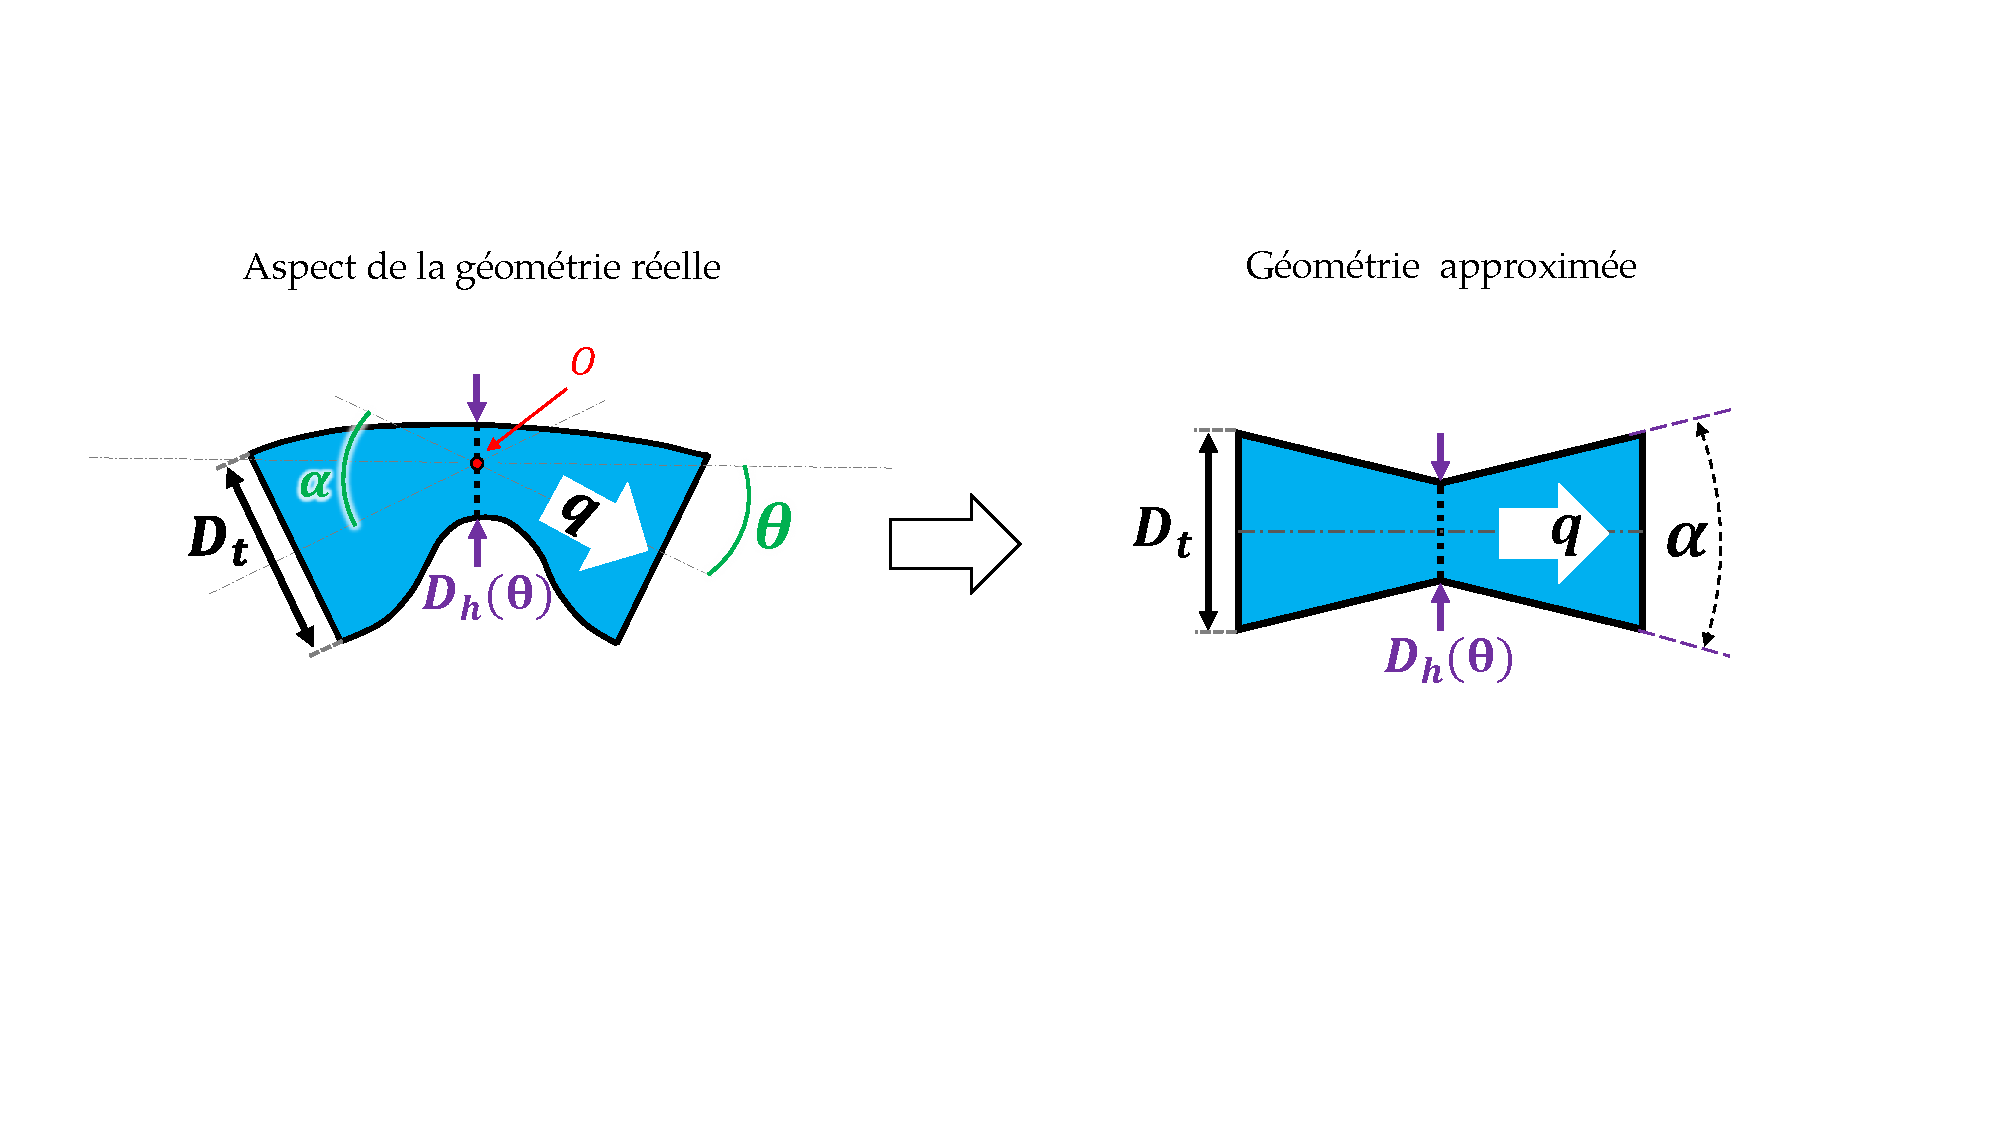
\includegraphics[trim={3cm 7cm 4.5cm 4cm},clip,width=0.9\textwidth]{../Chap5/Figure/geometrie_approx.pdf}
		\caption{Approximation de la géométrie de la section flambée d'un tube cylindrique}
		\label{fig:geometrie_approx}
	\end{center}
\end{figure}
%%%%%%%%%%%%%%%%%%%%%%%%%%%%%

Le phénomène de flambement dans les conduites flexibles est le plus souvent étudié dans un contexte de différence de pression entre l'intérieur et l'extérieur de la conduite \cite{Conrad1969,Heil1996,Ribeau1994,Elad1992}. En effet, lorsque cette différence est capable de déformer le tube, ce dernier peut flamber sous les forces de pression. Ces études sont le plus souvent appliquées aux veines du corps humain, dont la très faible raideur est fortement soumise aux différences de pression internes/externes à la veine \cite{Podoprosvetova2021,Nahar2019,Ghazy2018}. Elles visent à caractériser la déformation mécanique de la conduite sous les pressions environnantes. Pour notre part, nous cherchons à  l'inverse, à caractériser un écoulement sous la déformation de la conduite. Ce phénomène est perçu nocif dans les contextes applicatifs de la littérature et de ce fait, il est difficile d'en trouver une modélisation théorique, car les publications concernées cherchent à prévenir l'apparition du flambement. Le cas du flambement en flexion n'est ailleurs jamais mentionné.

Une solution simplifiée est d'approximer la section de passage flambée par une géométrie dont on peut trouver une valeur de $Cf$ dans la littérature. La géométrie de passage "réelle" en vue de coupe autour de la section flambée d'un tube flexible, ainsi que la géométrie approximée de cette section, sont schématisées sur la figure \ref{fig:geometrie_approx}. Le diamètre en entrée de la perturbation est $D_t$, le diamètre initial du tube. L'étranglement se fait jusqu'au diamètre hydraulique $D_h$ (éq. \ref{eq:Dh_definition}) de la section flambée.  La restriction ainsi créée s'approche d'une contraction conique, suivie d'une expansion conique de même angle $\alpha$. Le changement de direction joue lui aussi un rôle dans les PdC mais sera négligé dans un premier temps en considérant son influence faible devant la restriction de diamètre. Les outils de modélisation qui seront exposés dans ce chapitre peuvent s'appliquer à une approximation de modèle de PdC différente du choix que nous avons fait.

Nous allons dans un premier temps considérer la géométrie approximée de la figure \ref{fig:geometrie_approx} afin d'approcher analytiquement $Cf$ pour section flambée. Les études empiriques de Gibson ont permis d'établir un modèle analytique de $Cf$ pour la géométrie approximée qu'on présente à la figure \ref{fig:geometrie_approx}\cite{Gibson1910, Idelcik1986, CRANECO1982}.
%%%%%%%%%%%%%%%%%%%%%%%%%%%%%%%%
\begin{align}
\Lambda _ c & = 
    \begin{cases}
	\biggl(1-\frac{S_r}{S_l}\biggr)^2\cdot\ 2.6\sin\biggl(\frac{\alpha}{2}\biggr) & \text{pour} ~~0<\alpha<\ang{45} \\
	\biggl(1-\frac{S_r}{S_l}\biggr)^2 & \text{pour}~~\ang{45}<\alpha<\ang{180} \\
    \end{cases}
\label{eq:Lambda_retrecissement}\\
\Lambda _ e & = 
    \begin{cases}
	0.5\biggl(1-\frac{S_r}{S_l}\biggr)^{0.75}\cdot\ 1.6\sin\biggl(  \frac{\alpha}{2}\biggr) & \text{pour} ~~0<\alpha<\ang{45} \\
	0.5\biggl(1-\frac{S_r}{S_l}\biggr)^{0.75}\cdot\ \sqrt{\sin\biggl(  \frac{\alpha}{2}\biggr)} & \text{pour}~~\ang{45}<\alpha<\ang{180} \\
    \end{cases}
\label{eq:Lambda_elargissement}
\end{align} 
%%%%%%%%%%%%%%%%%%%%%%%%%%%%%%%%
\begin{equation}
Cf = \frac{\Delta p}{q^2} = \biggl(\frac{8\rho}{\pi {D_h}^4}\biggr)\Lambda
\label{eq:Cf_definition2}
\end{equation}	

$C_f$ est défini par l'équation \ref{eq:Cf_definition2}. La seule inconnue est $\Lambda$ et ce coefficient dépend seulement de la géométrie de la perturbation. Les résultats issus des études de Gibson sont présentés dans les équations \ref{eq:Lambda_retrecissement} et \ref{eq:Lambda_elargissement}. $\Lambda_r$ et $\Lambda_e$ sont respectivement les coefficients de perturbation hydraulique induits par le rétrécissement et l'élargissement de la conduite. ${S_r}$ et ${S_l}$ sont les surfaces respectives de la section réduite et de la section large. Enfin, $\alpha$ représente l'angle du cône de rétrécissement, et est identique à l'élargissement. Gibson a identifié, que pour une conduite circulaire, les PdC atteignent un maximum lorsque $\alpha=\ang{63}$ et un minimum lorsque $\alpha=\ang{13.5}$ \cite{Gibson1910}. Dans notre cas, cet angle sera dépendant de l'angle de flexion $\theta$ du tube et sera d'autant plus important que celui-ci augmente. Il sera pris égal à $2\theta$ en première approximation, comme le montre la figure \ref{fig:geometrie_approx}. Le coefficient Cf s'exprime alors pour la géométrie approximée d'une section de tube flambée par :
\begin{equation}
C_{f,VH}  = 
	\frac{4\ \rho}{\pi^2\ {D_h}^4}\ 
\Biggl[ 1.6\biggl(1-\frac{{D_h}^2}{{D_t}^2}\biggr)^{0.75} + 
		5.2\biggl(1-\frac{{D_h}^2}{{D_t}^2}\biggr)^{2} 
\Biggr] \sin(\theta)
\label{eq:Cf_Gibson_45deg}
\end{equation} 
    %/////////////////////////////////////////////
    \subsection{Critères de conception}
    \label{subsec:5.1.3 - Criteres de conception}
    %/////////////////////////////////////////////        
Un rapport $(r_{Cf})_{min} \ge 10$ est nécessaire pour assurer le bon fonctionnement des VH. En fixant alors le diamètre $D_t$ du tube, l'équation \ref{eq:Cf_Gibson_45deg} donne le diamètre de fermeture $D_{hf}$ que doit avoir la section flambée pour assurer $(r_{Cf})_{min}$.

À présent, il faut établir un critère de sélection afin de déterminer $D_t$. Plusieurs facteurs peuvent conditionner ce choix. L'évolution de $\theta$ en fonction de $x_m$, illustrée sur la figure \ref{fig:(theta&a)_vs_xm_avec_et_sans_gaine_tot}, montre que l'amplitude du déplacement de la masse doit être suffisante pour plier le tube sur la plage d'angle $\Delta\theta$ assurant l'ouverture et la fermeture de la VH. La valeur de $|x_0|<1$mm est connue d'après les simulations du chapitre \ref{ch:2_Modelisation et simulation du systeme}. Par conséquent, l'amplitude $\Delta \theta$ pour plier la valve sera uniquement dépendante du bras de levier de pliage $a$. D'après l'équation \ref{eq:OB+GPA+VH+piston} l'impact de la rigidité du tube sur l'OB est inversement proportionnel à $a$ et donc il faudrait minimiser cette distance pour limiter l'impact de la raideur $K_{VH}$. Cela revient à minimiser $\Delta \theta$. C'est donc dans ce sens qu'il faut faire évoluer les paramètres matériau et géométriques du tube afin de minimiser $K_{VH}$.

D'autre part, on peut s'appuyer sur l'équation \ref{eq:Cf_definition} et sur l'ordre de grandeur de $D_h$ et $D_t$ afin d'estimer leur influence sur l'évolution de $C_{f,VH}$. Pour caractériser la capacité d'étranglement à la section flambée lors de la flexion du tube, on introduit le rapport de fermeture $f_D$ défini tel que :
\begin{equation}
	f_D = \frac{D_h}{D_t}
	\label{eq:f_D_definition}
\end{equation}
L'équation \ref{eq:Cf_Gibson_45deg} peut alors être exprimée en fonction de $f_D$ comme suit :
\begin{equation}
C_{f,VH}\ =\ \frac{4\rho\sin(\theta)}{\pi^2\ {D_t}^4}\ g(f_D)
\label{eq:Cf_Gibson_g(fD)}\\
\end{equation}
Où $g(f_D)$ est une fonction de $f_D$  et exprimée par l'équation \ref{eq:g(fD)_definition}
\begin{equation}
g(f_D)  \ =\ \dfrac{1}{{f_D}^4} \biggl(1.6(1-{f_D}^2)^{0.75} + 5.2(1-{f_D}^2)^2\biggr)
\label{eq:g(fD)_definition}
\end{equation}
On sait $f_D\in]\ 0\ ;\ 1\ ]$ et, par extension, on sait que $g(f_D)$ sera bornée. La figure \ref{fig:g(fD)} montre alors l'évolution de $g(f_D)$ pour $f_D\in[\ 0.3\ ;\ 1\ ]$. 
%%%%%%%%%%%%%%%%%%%%%%%%
\begin{figure}[!htb]
	\begin{center}
		\captionsetup{justification=centering}
		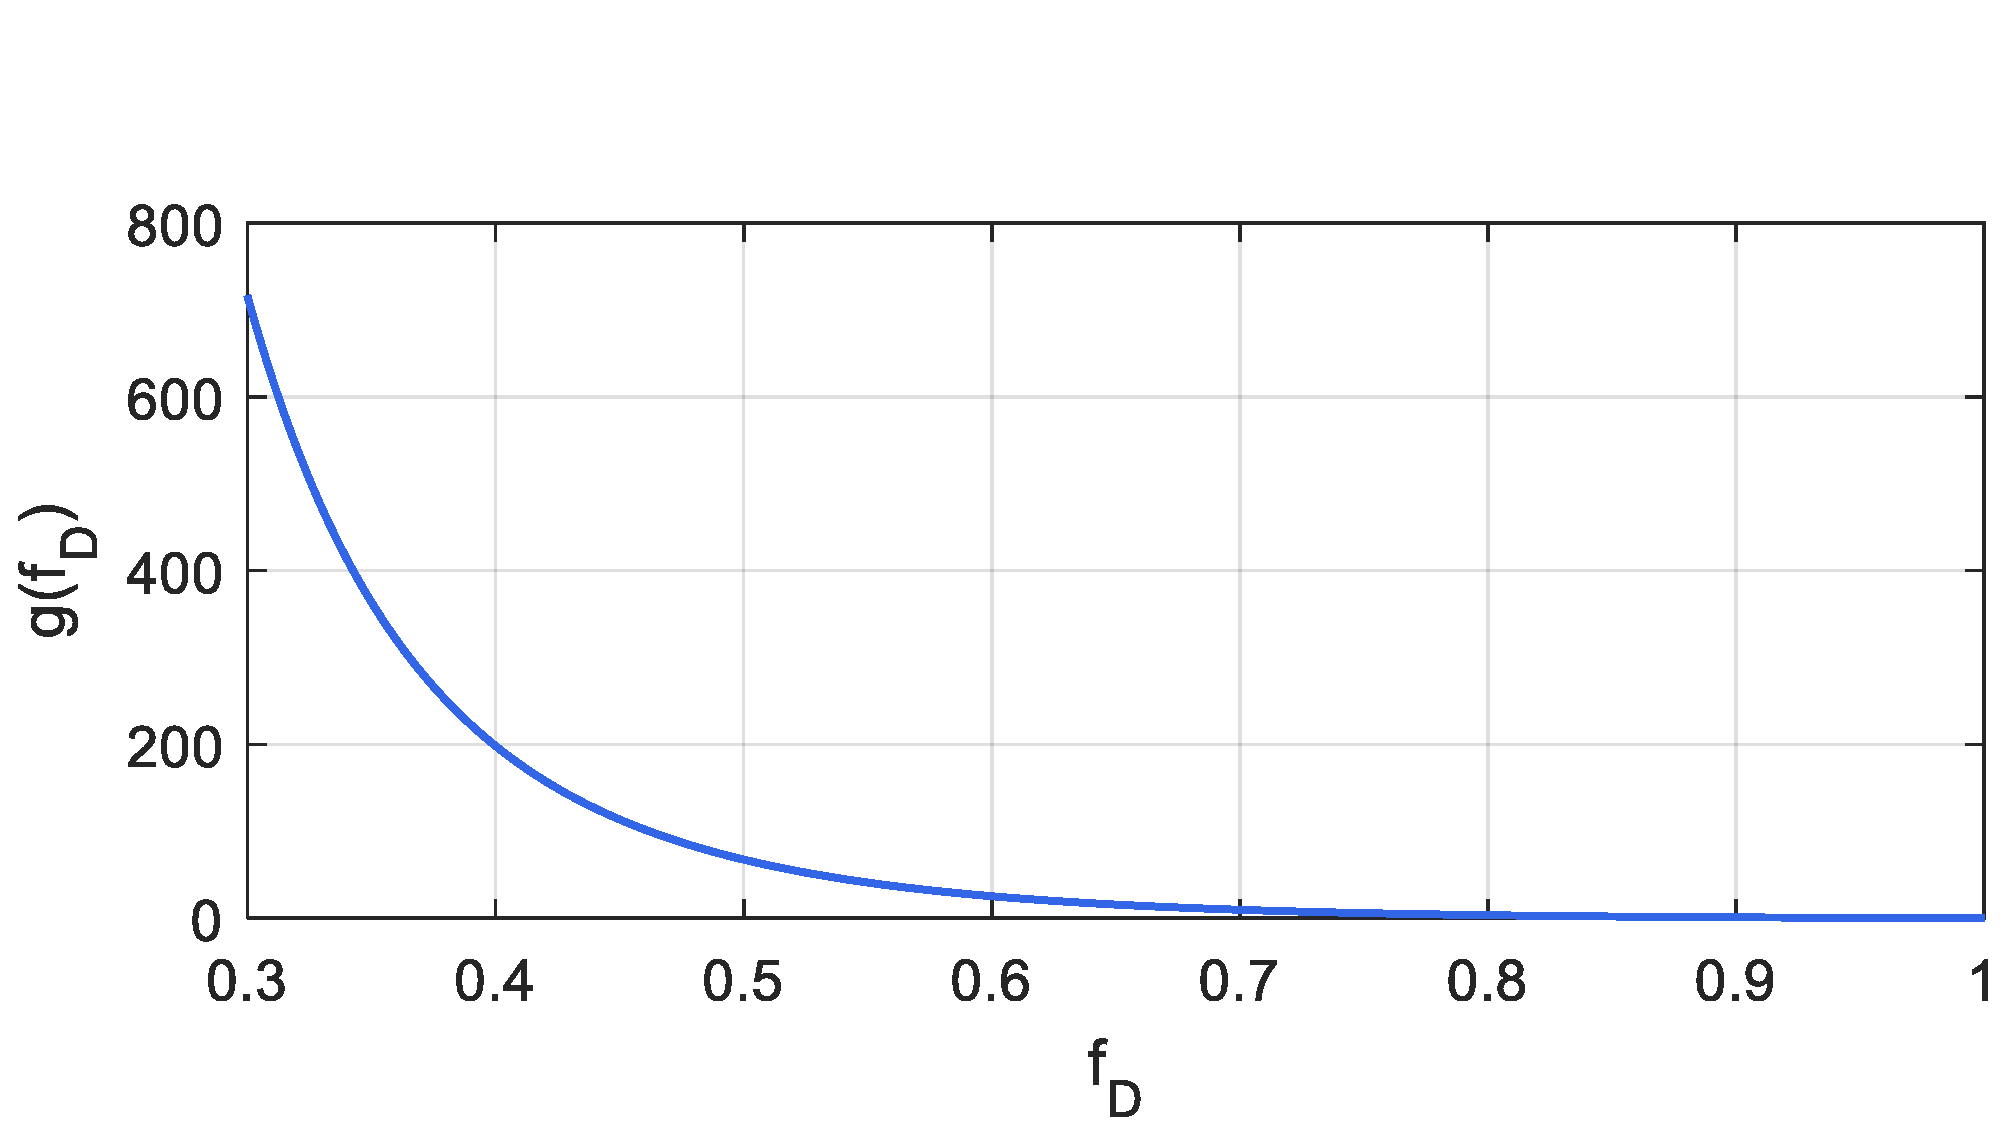
\includegraphics[trim={0cm 0cm 0cm 3cm},clip,width=0.8\textwidth]{../Chap5/Figure/g(fD).pdf}
		\caption{Évolution de $g(f_D)$ pour$f_D\in[\ 0.3\ ;\ 1\ ]$ }
		\label{fig:g(fD)}
	\end{center}
\end{figure}
%%%%%%%%%%%%%%%%%%%%%%%%%%%%%
$g(f_D)$ augmente alors lorsque $f_D$ diminue. Cela signifie que lorsque $D_h$ diminue, $C_{f,VH}$ augmente. Le tube à concevoir doit donc pouvoir offrir une diminution de $f_D$ suffisamment importante afin que la VH puisse générer un rapport de fermeture hydraulique $(r_{Cf}) \ge 10$.
Les 5 paramètres susceptibles d'affecter ce CdC sont : le module d'Young $E_{t}$ et le coefficient de Poison $\nu_t$ du matériau, le diamètre initial $D_t$, l'épaisseur $th_t$, ainsi que la longueur $L_t$ du tronçon de tube. De fait, un modèle EF dépendant de ces paramètres est établi, pour étudier leur influence sur l'évolution de $f_D$ et, par extension, sur l'évolution de $C_{f,VH}$.

Il est à noter sur la figure \ref{fig:g(fD)} que la variation de $C_{f,VH}$ devient significative pour des rapports $f_D$ inférieurs à 0.7. Pour profiter d'une variation de $C_{f,VH}$ importante sur une plage d'angle $\Delta\theta$ la plus faible possible, il sera pertinent de fixer un angle de flexion $\theta_0$ non nul en position ouverte.
%/!\/!\/!\/!\/!\/!\/!\/!\/!\/!\/!\/!\/!\/!\/!\/!\/!\/!\/!\/!\/!\/!\/!\/!\ 
\section{Étude EF des tubes}
\label{sec:5.2}
%/!\/!\/!\/!\/!\/!\/!\/!\/!\/!\/!\/!\/!\/!\/!\/!\/!\/!\/!\/!\/!\/!\/!\/!\ 
    %/////////////////////////////////////////////
    	\subsection{Présentation du modèle}
    	\label{subsec:5.2.1 - Présentation du modèle EF}
    %/////////////////////////////////////////////
L'étude EF a été réalisée avec l'outil \emph{ANSYS APDL mechanical}. Le modèle ayant servi à l'étude, ainsi que ses conditions limites, sont illustrés sur la figure \ref{fig:Modele_EF_presentation}. Il se compose essentiellement d'une portion de cylindre creux. L'étude a été réalisée avec l'élément SHELL63. La géométrie du tube a été définie par sa longueur $L_t$, son diamètre intérieur $D_t$ et son épaisseur $th_t$. Le matériau utilisé est élastique isotrope homogène et défini par son module d'Young $E_t$ et son coefficient de Poisson $\nu_t$. Les plans $S_1$ et $S_2$ aux extrémités du tube représentent la jonction avec les gaines rigides des parties fixes et mobiles représentées en rouge sur la figure \ref{fig:detail_flambement_MDOB}.
%%%%%%%%%%%%%%%%%%%%%%%%%%%%%%%%%
\begin{figure}[!htbp]
	\begin{center}
		\captionsetup{justification=centering}
		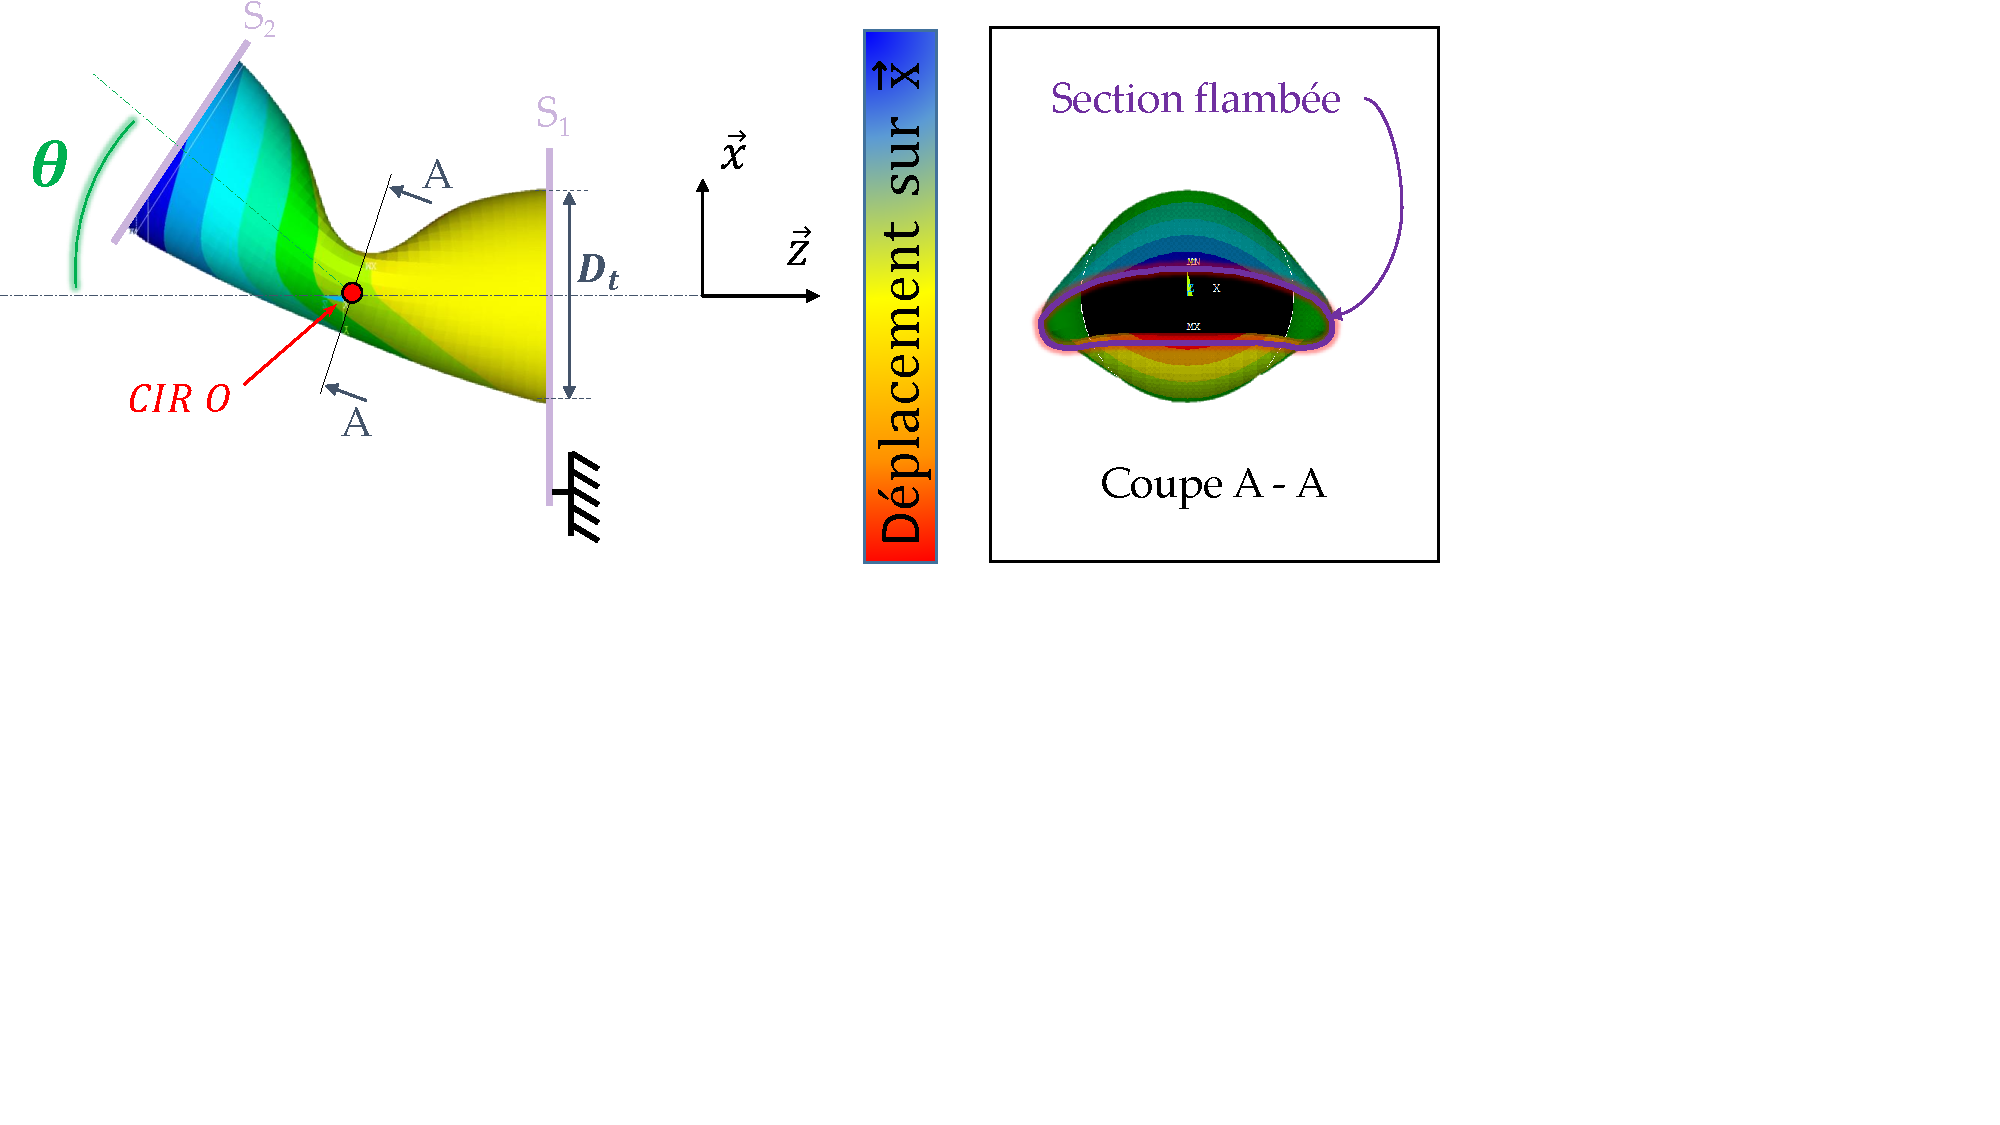
\includegraphics[trim={0cm 9cm 9cm 0cm},clip,width=0.7\textwidth]{../Chap5/Figure/presentation_modele_EF.pdf}
		\caption{Modèle EF d'un tube flexible sous un angle $\theta$ imposé}
		\label{fig:Modele_EF_presentation}
	\end{center}
\end{figure}  
%%%%%%%%%%%%%%%%%%%%%%%%%%%%%%%%%  

Les hypothèses pour la résolution du modèle sont les suivantes :
\begin{itemize}[label=$\circ$]
\item Les sections $S_1$ et $S_2$ sont rigides.
\item La résolution se fait en grands déplacements.
\end{itemize} 
Les déplacements imposés sont les suivants :
\begin{itemize}[label=$\bullet$]
\item Les n\oe{}uds appartenant au plan $S_1$ sont fixes dans l'espace. 
\item L'angle $\theta$ est imposé et défini comme l'angle formé par l'intersection des deux axes des sections $S_1$ et $S_2$. On peut retrouver sur la figure \ref{fig:theta_impose} le détail du déplacement imposé aux n\oe{}uds du plan $S_2$ afin que le flambement se produise au centre de la longueur $L_t$. Le centre \emph{O} est immobile dans l'espace et se trouve au centre du cylindre non déformé.
\item Les conditions initiales pour chaque incrément d'angle sont issues de la position d'équilibre finale de la résolution du modèle avec l'incrément d'angle précédent.
\end{itemize}
%%%%%%%%%%%%%%%%%%%%%%%%%%%%%%%%%%%%
\begin{figure}[!htbp]
\begin{center}
    \captionsetup{justification=centering}
	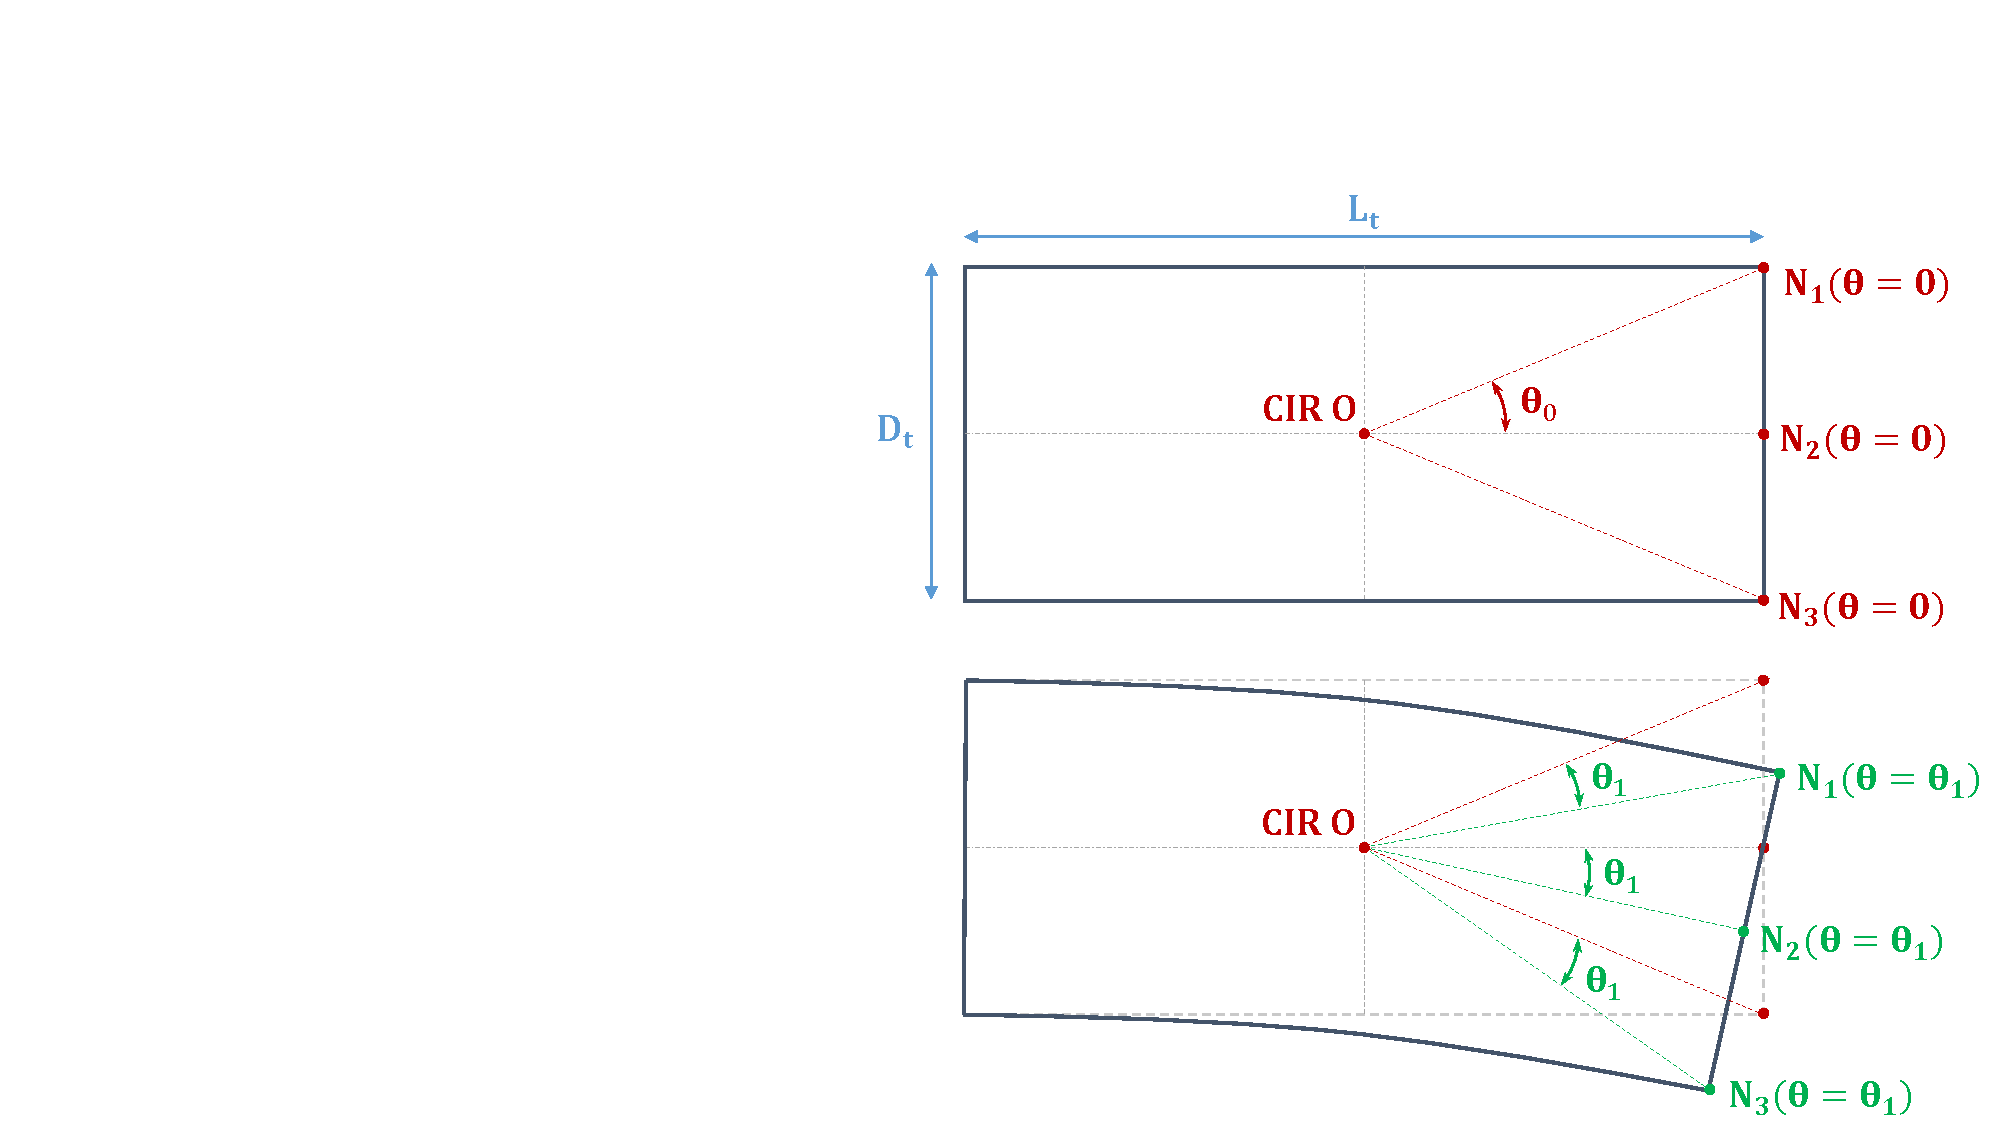
\includegraphics[trim={14.5cm 0cm 0cm 4cm},clip,width=0.7\textwidth]{../Chap5/Figure/theta_impose.pdf}
	\caption{Origine de l’angle $\theta$}
	\label{fig:theta_impose}
\end{center}	
\end{figure} 
%%%%%%%%%%%%%%%%%%%%%%%%%%%%%%%%%%%% 
%%%%%%%%%%%%%%%%%%%%%%%%%%%%%%%%%%%%
\begin{figure}[!htbp]
\begin{center}
    \captionsetup{justification=centering}
	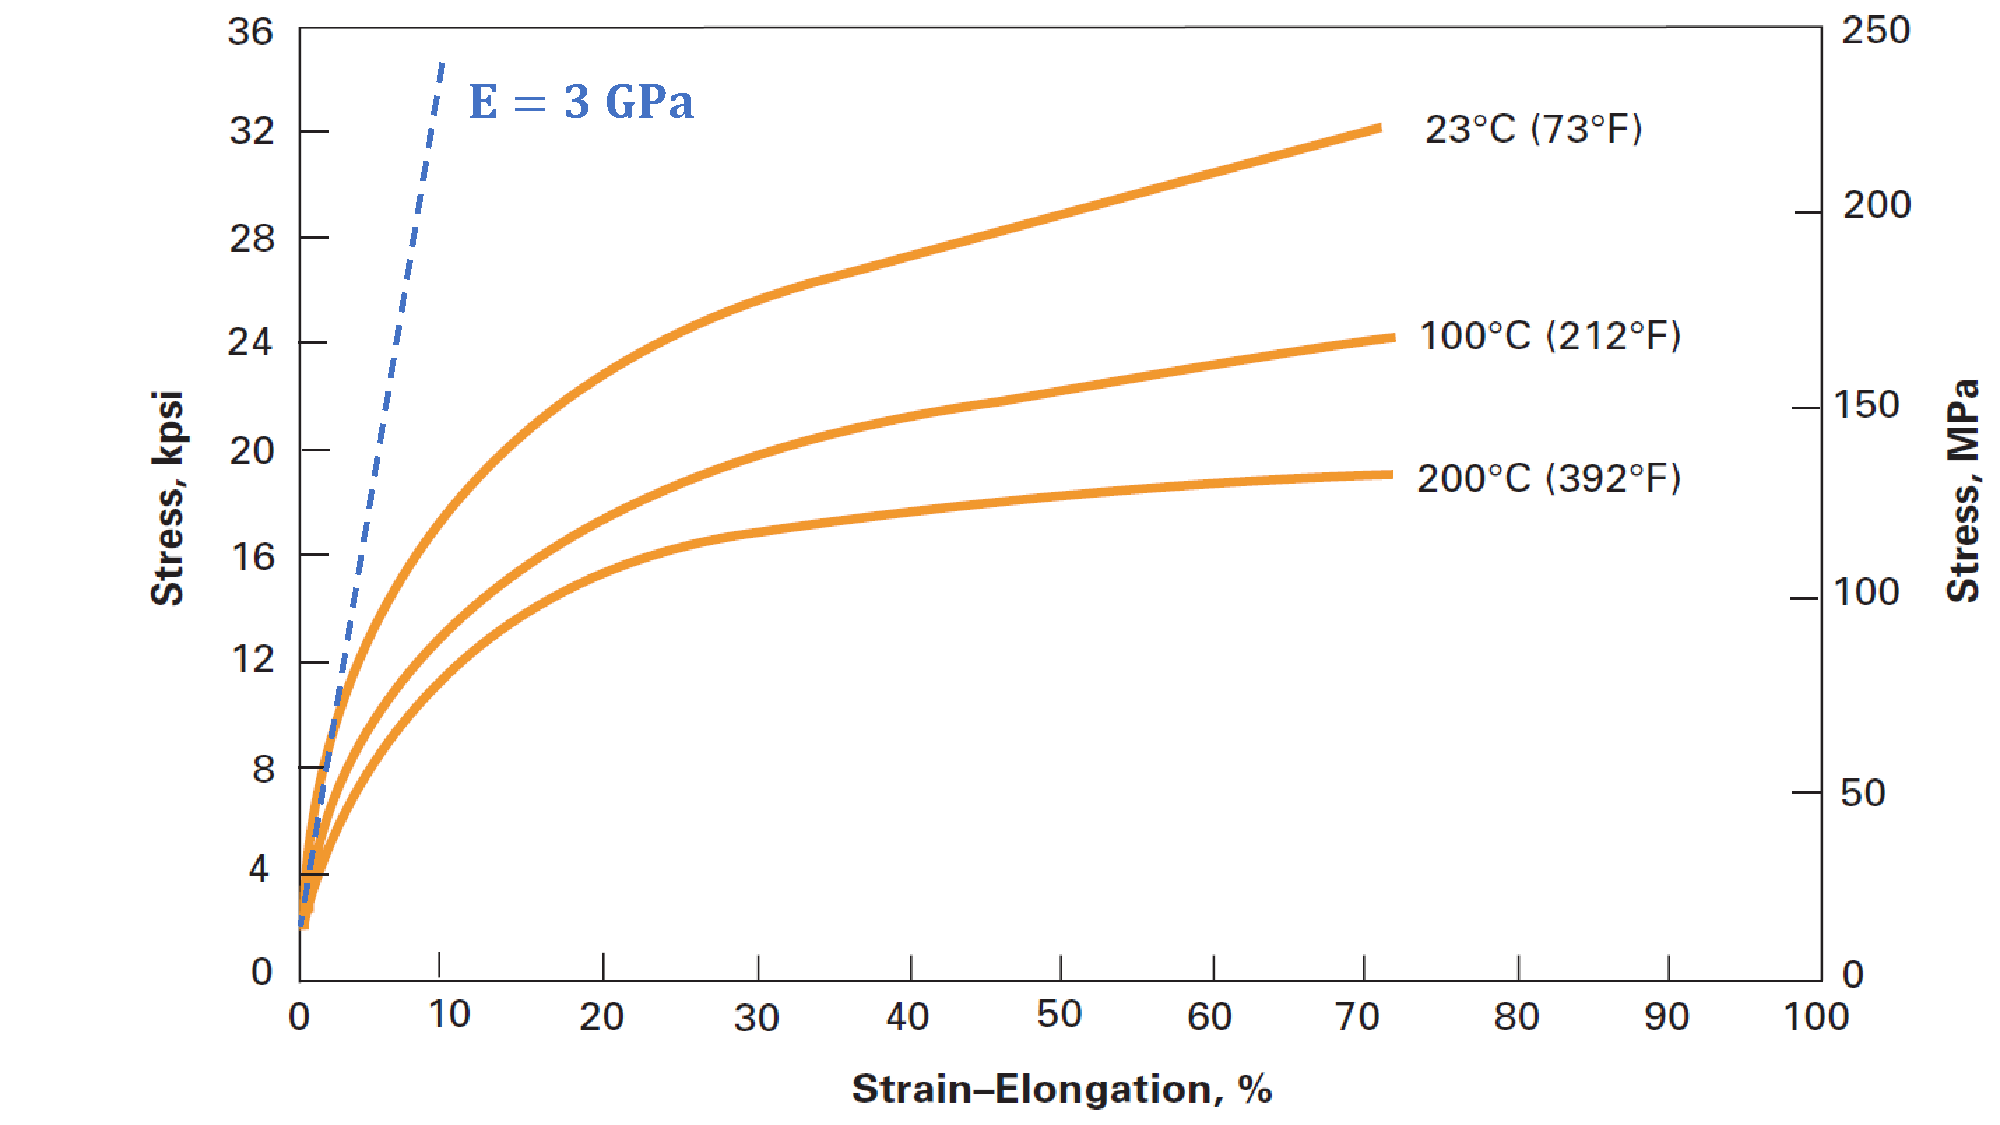
\includegraphics[trim={2cm 0cm 0cm 0cm},clip,width=0.8\textwidth]{../Chap5/Figure/Dupont_kapton.pdf}
	\caption{Courbe de contraintes-déformations en traction de kapton HN \cite{Dupont2012}}
	\label{fig:Dupont_kapton}
\end{center}	
\end{figure} 
%%%%%%%%%%%%%%%%%%%%%%%%%%%%%%%%%%%%      
Le choix de matériau a été fixé durant l'étude expérimentale (sec. \ref{subsec:4.2.2_Choix du matériau}). Le comportement élastique du matériau kapton choisi est présenté sur la figure \ref{fig:Dupont_kapton} issu des données constructeur pour trois températures de recuit. Le kapton possède un comportement matériau assouplissant, et donc, son module d'Young est décroissant en fonction du niveau de contraintes. Afin de simplifier la résolution du modèle EF, il se place dans le cas le plus défavorable. Par conséquent, le module d'élasticité est constant et les déformations sont considérés faibles. Avec les données techniques du kapton, $E_t = 3$GPa. Aussi, $\nu_t = 0.3$, une valeur récurrente pour les polymères. Le coefficient de Poisson ne devrait pas avoir une influence significative, au vu des très faibles épaisseurs qui seront considérées. Par ailleurs, le matériau est supposé isotrope, ce qui peut être éloigné du tube réalisé par enroulement en spirale (cas des essais expérimentaux).

Afin de déterminer l'évolution de $D_h$, on relève la position des n\oe{}uds se trouvant sur le périmètre formant le plan de symétrie vertical passant par \emph{O} lorsque le tube est horizontal. Ce périmètre est illustré sur la coupe A-A de la figure \ref{fig:Modele_EF_presentation}. Connaissant les coordonnées du nuage de points ainsi formé, on applique la formule énoncée à l'équation \ref{eq:Dh_definition} pour extraire $D_h$ pour chaque incrément de $\theta$.

De plus, il est possible d'extraire des simulations, l'énergie de déformation élastique $W_t$ emmagasinée dans le tube fléchi. Connaissant le déplacement imposé, la rigidité $K_{VH}$ peut être évaluée d'après l'équation \ref{eq:K_HV = 1/thetadW/dtheta}.
\begin{equation}
 	K_{VH} = \frac{1}{\theta} \cdot \frac{dW_t}{d\theta}
 	\label{eq:K_HV = 1/thetadW/dtheta}
\end{equation}   
    %/////////////////////////////////////////////
    	\subsection{Influence des paramètres géométriques du tube}
    	\label{sec:5.2.2 - Impact des parametres geometriques du tube}
    %/////////////////////////////////////////////	
On souhaite déterminer l'influence des paramètres $D_t$, $L_t$ et $th_t$ sur l'évolution de $f_D$. On va se servir d'une matrice de jeux de paramètres de dimension $3^2$, où $3^2$ est le nombre de simulations à réaliser avec un jeu de paramètres ($D_t$ x $L_t$ x $th_t$) différent pour chacune d'elles. La matrice de paramètres est présentée dans le tableau \ref{tab:jeux de parametres de simulations EF}
%%%%%%%%%%%%%%%%%%%%%%%%%%%%%%%%%%%%	
\begin{table}[!htbp]
	\centering
		\begin{tabular}[t]{|c|c|c|c|}
\cline{2-4}
\multicolumn{1}{c|}{}	&
$D_t$ [mm]				&
$th_t$ [$\micro$m]		& 
$L_t$ [mm] \\
\cline{2-4} \hline
$D_t$ [mm]			& 0.42 & 0.5 & 0.62 	\\
\hline
$th_t$ [$\micro$m]	& 15   & 25   & 40  	\\
\hline
$L_t$ [mm]    	    & 1    &2     & 3.5		\\
\hline
		\end{tabular}
        \caption{Matrice de paramètres}
        \label{tab:jeux de parametres de simulations EF}
\end{table}        
%%%%%%%%%%%%%%%%%%%%%%%%%%%%%%%%%%%%	

L'étude expérimentale des tubes kapton a montré que le tube T50 (tab. \ref{tab:dim_tube_statique}) non plastifié admet une raideur $K_{VH}$ (fig \ref{fig:resultats_essais_statique_VH_tous}) acceptable pour la limite d'admissibilité de l'OB fabriqué (fig \ref{fig:(K_VH)_max(a)_et_Deltatheta_pour_bistabilite}). C'est pourquoi les trois diamètres initiaux $D_t$ choisis pour les simulations se situent autour de $0.5$mm.
    		%*************	
 		\subsubsection{Aspects hydrauliques}
    		%************* 	
On cherche à maximiser $\Delta f_D$ sur une plage d'angle $\Delta \theta$ la plus faible possible. La figure \ref{fig:prospection_fD} montre alors les résultats des simulations EF concernant l'évolution de $f_D(\theta)$. Chaque quadrant montre les simulations réalisées en fixant deux des paramètres $D_t$, $th_t$ et $L_t$, pour isoler l'influence du troisième. L'angle de flambement est repéré pour chaque simulation sur l'axe des abscisses. Face au besoin, ces résultats montrent la nécessité de minimiser l'épaisseur, en maximisant le diamètre du tube. On note que la hauteur du saut de $f_D$ lors de l'apparition du flambement n'est que peu significativement impactée par ces deux paramètres, contrairement à la longueur $L_t$. En augmentant cette-dernière, le flambement apparaît pour des angles plus élevés et induit une hauteur de saut de $f_D$ plus importante après l'apparition du phénomène. En revanche, on s'aperçoit qu'après flambement $f_D$ tend vers la même valeur, indépendamment de $L_t$.
%%%%%%%%%%%%%%%%%%%%%%%%%
\begin{figure}[!htbp]
	\begin{center}
		\begin{subfigure}[b]{0.49\textwidth}
			\captionsetup{justification=centering}
			\captionsetup{justification=centering}
			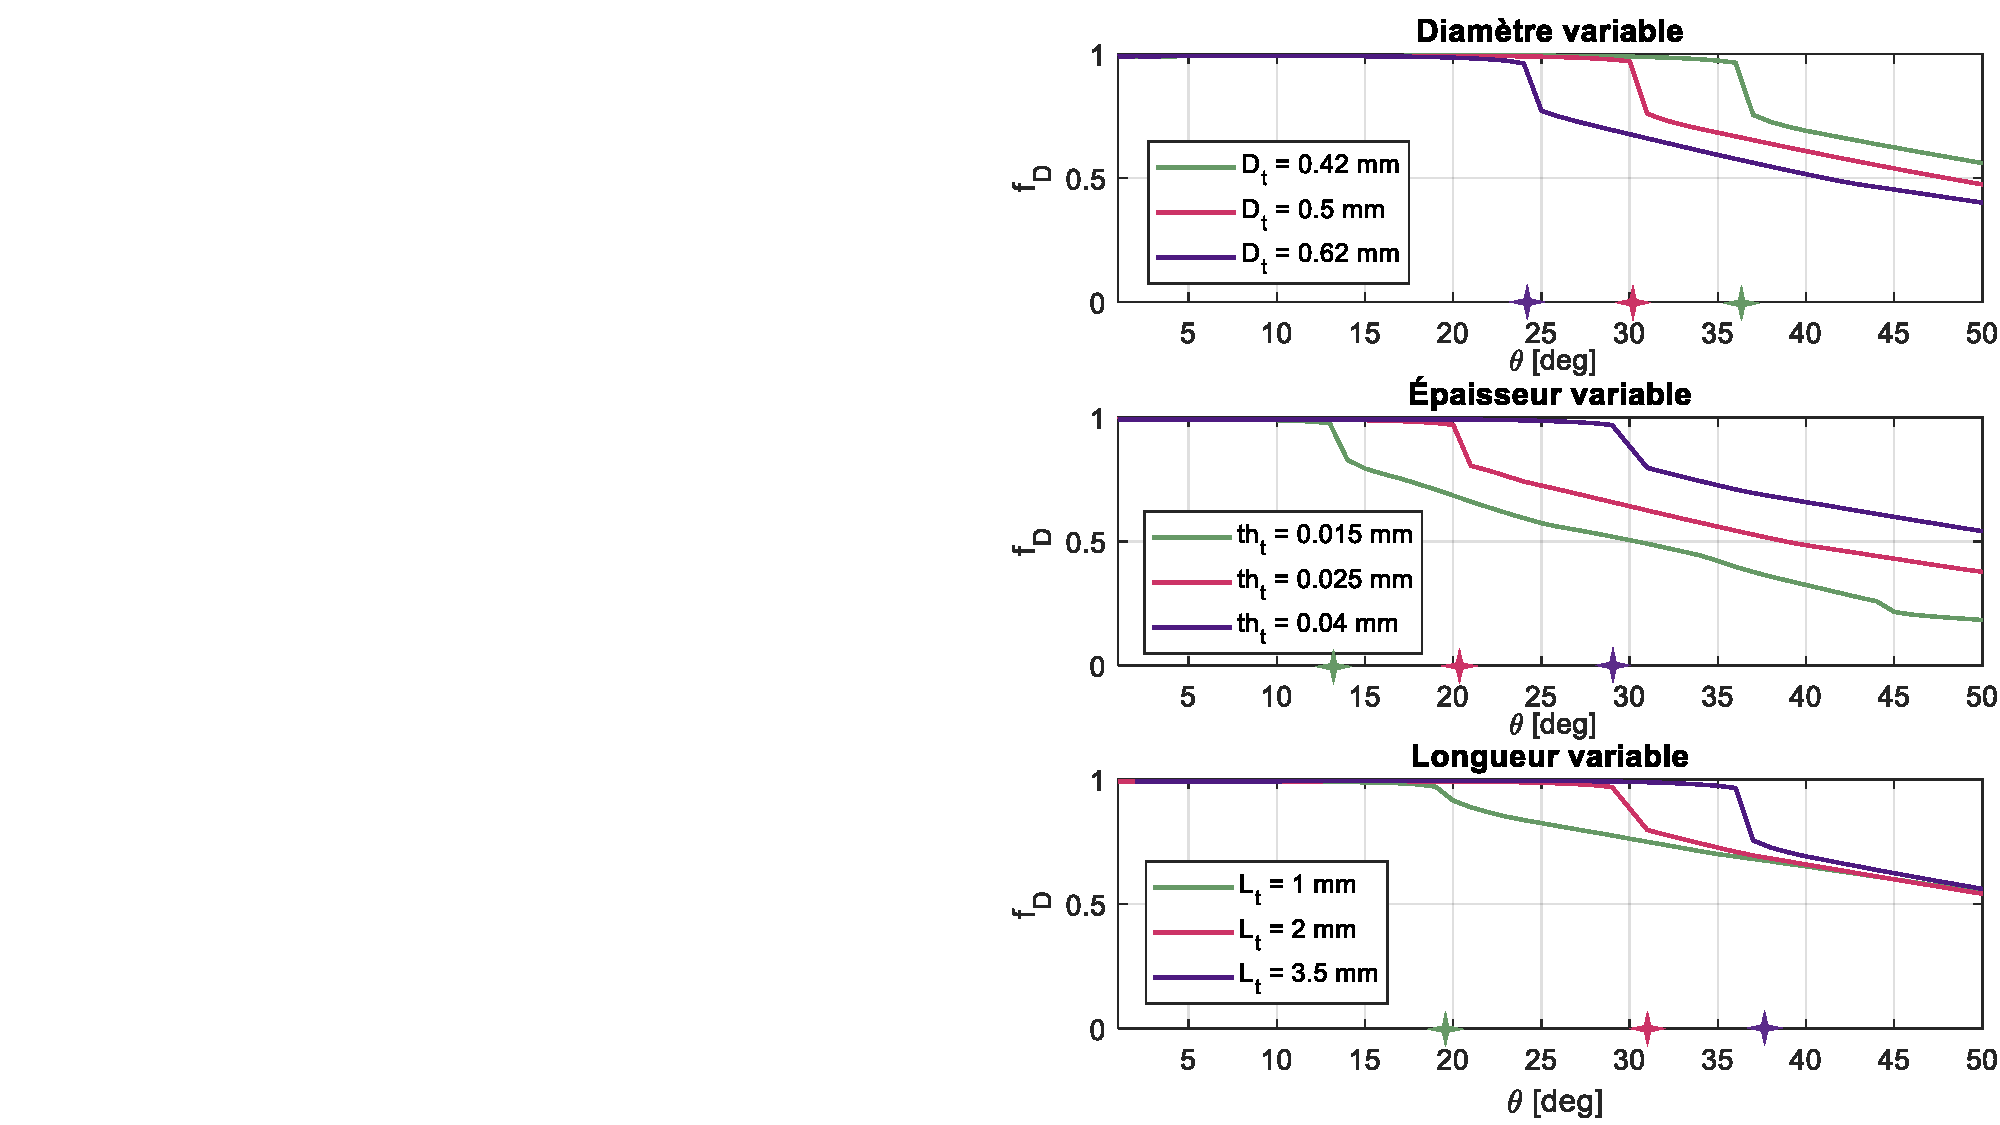
\includegraphics[trim={17cm 0cm 0cm 0cm},clip,width=\textwidth]{../Chap5/Figure/prospection_fD_L&R&thvar.pdf}
			\caption{Influence de l'épaisseur, de la longueur et du diamètre initial du tube sur $f_D(\theta)$}
			\label{fig:prospection_fD}
		\end{subfigure}
		\hfillx
		\begin{subfigure}[b]{0.49\textwidth}
			\captionsetup{justification=centering}
			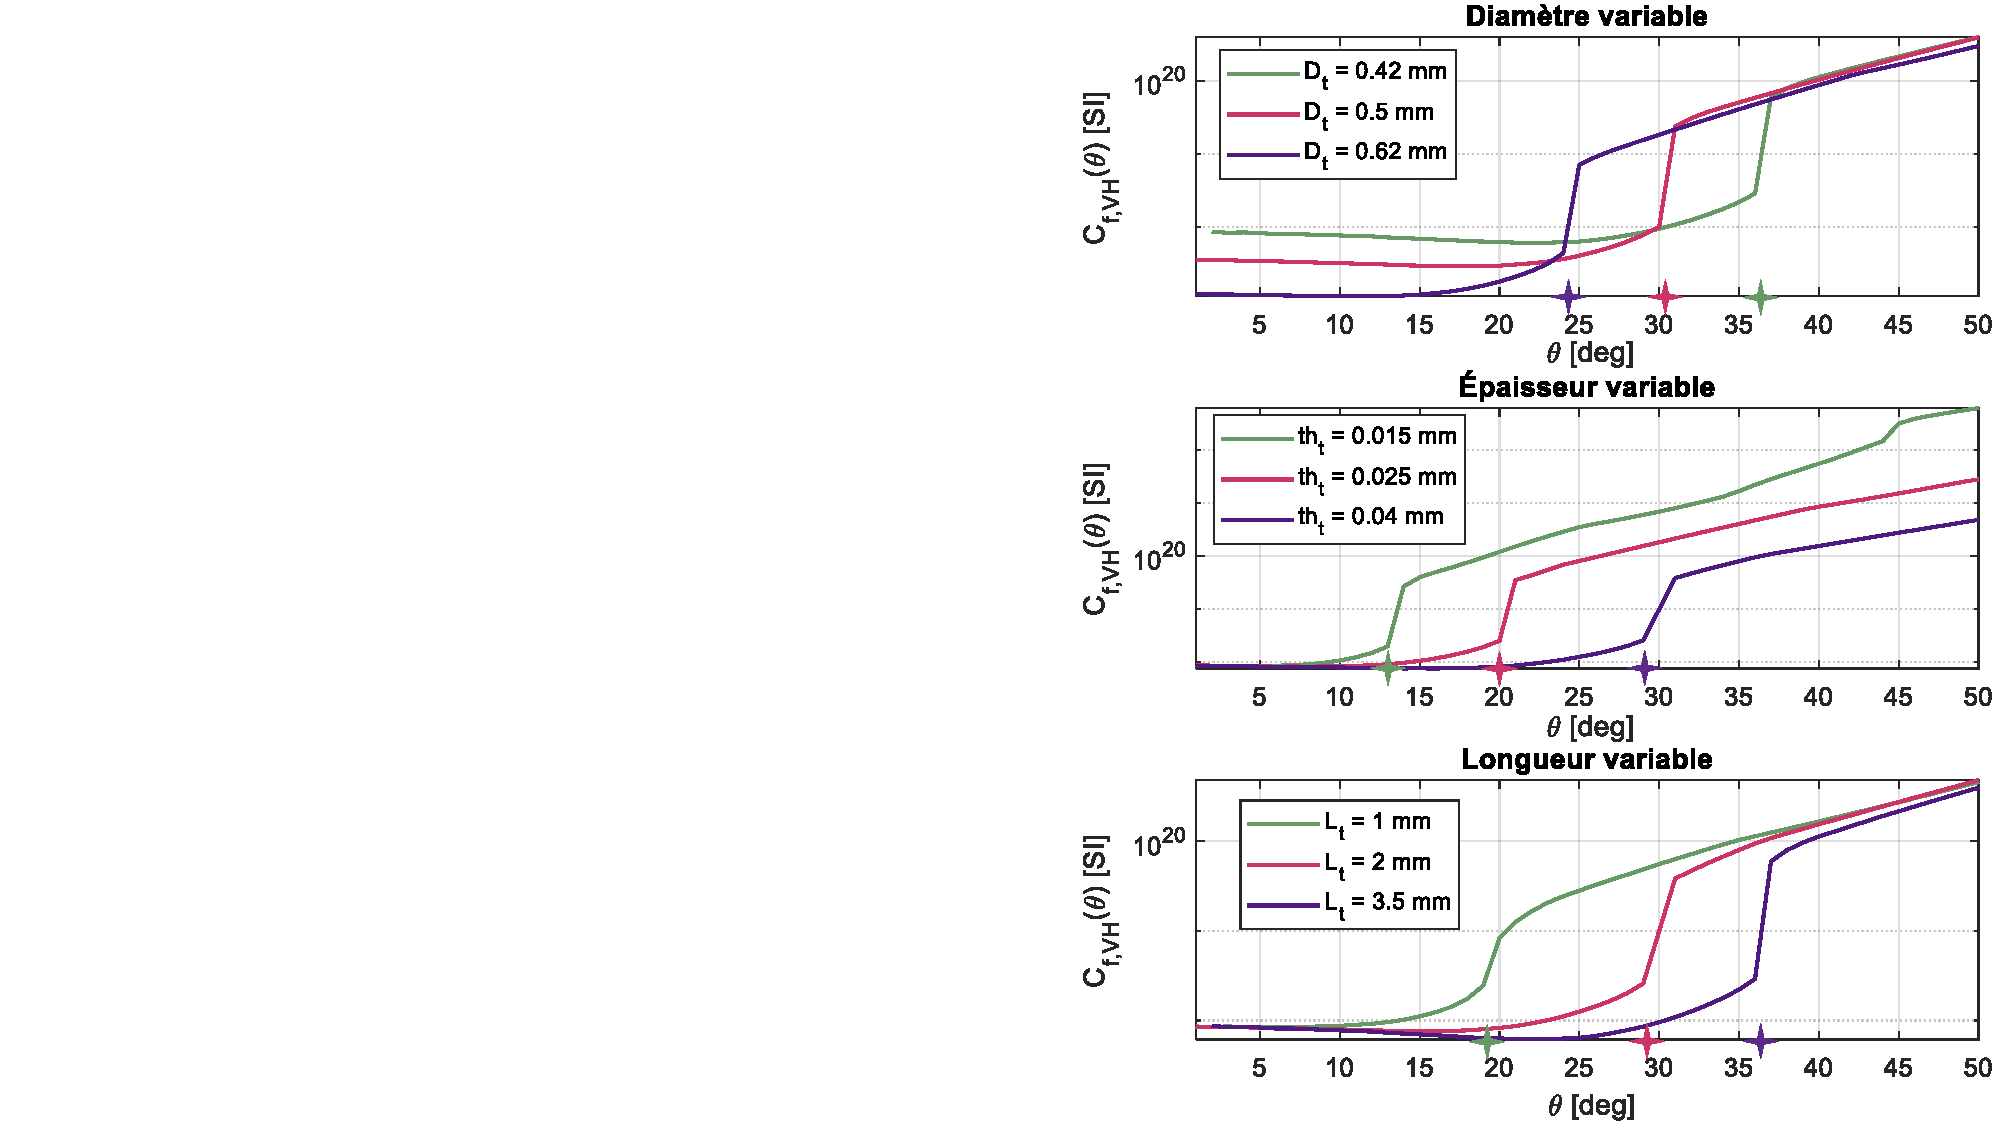
\includegraphics[trim={17cm 0cm 0cm 0cm},clip,width=\textwidth]{../Chap5/Figure/prospection_Cf_L&R&thvar.pdf}
			\caption{Influence de l'épaisseur, de la longueur et du diamètre initial du tube sur $C_{f,VH}(\theta)$}
			\label{fig:prospection_Cf}
		\end{subfigure}
		\caption{Résultats des simulation EF sur les aspects hydrauliques}
		\label{fig:prospection_(fD+Cf)}
	\end{center}
\end{figure}
%%%%%%%%%%%%%%%%

À l'aide de l'équation \ref{eq:Cf_Gibson_g(fD)}, on trace aussi les courbes de l'évolution de $C_{f,VH}$ en fonction de $\theta$ pour ces mêmes simulations sur la figure \ref{fig:prospection_Cf}. Afin de maximiser la variation $\Delta C_{f,VH}$ pour un $\Delta \theta$ minimal, les tendances d'évolution avec $L_t$, $D_t$ et $th_t$ devront logiquement être les mêmes que précédemment pour $f_D$.

Un angle faible est bénéfique pour réduire les PdC dans la branche qui actionne. En revanche, il serait bénéfique d'exploiter les tubes en position ouverte avec une pré-contrainte d'angle fixe et proche de l'angle de flambement $\theta _f$. On pourra alors profiter du phénomène afin de diminuer $\Delta \theta$ car $\Delta C_{f,VH}$ est très faible sur la plage d'angle $[0;\theta _f]$. Un compromis est donc à déterminer pour l'angle d'ouverture de la VH.

On relève que $(r_{Cf})_{min}$ est atteignable pour tous les tubes qui ont été simulés. Si on se place à la limite du flambement, et qu'on compare $C_{f,VH}$ avant et après le phénomène, on reste dans le respect du CdC hydraulique. Une plage $\Delta \theta \approx \ang{1-2}$ serait alors suffisante avec les tubes simulés. La restriction hydraulique dans les tubes de très faibles diamètres semble très importante. En effet, l'ordre de grandeur de $C_{f,VH}$ est 4 à 5 fois supérieure à celui que nous avons relevé dans les simulations de pré-dimensionnement de la figure \ref{fig:simu_pos_debit_Cf_pression_1CYCLE}. Cette différence est induite par le terme ${D_t}^4$ qu'on retrouve au dénominateur de la formule définissant $C_{f,VH}$. On peut en déduire qu'il est possible d'augmenter $D_t$ par simulations itératives, en veillant à respecter $(r_{Cf})_{min}=10$. Ce résultat est positif du point de vue de la facilité d'intégration technologique, car à faibles diamètres, les montages hydrauliques expérimentaux deviennent plus complexes à manipuler. Il faudra cependant garder une attention sur la raideur du tube qui, d'après les résultats expérimentaux (fig. \ref{fig:resultats_essais_statique_VH_tous}), devient plus importante avec l'augmentation du diamètre. Ce résultat sera par ailleurs confirmé par l'étude théorique qui suit.
%%%%%%%%%%%%%%%%%%%%%%%%%%%%%%%%%%%%%	
%\begin{figure}[!htb]
%\begin{center}
%    \captionsetup{justification=centering}
%	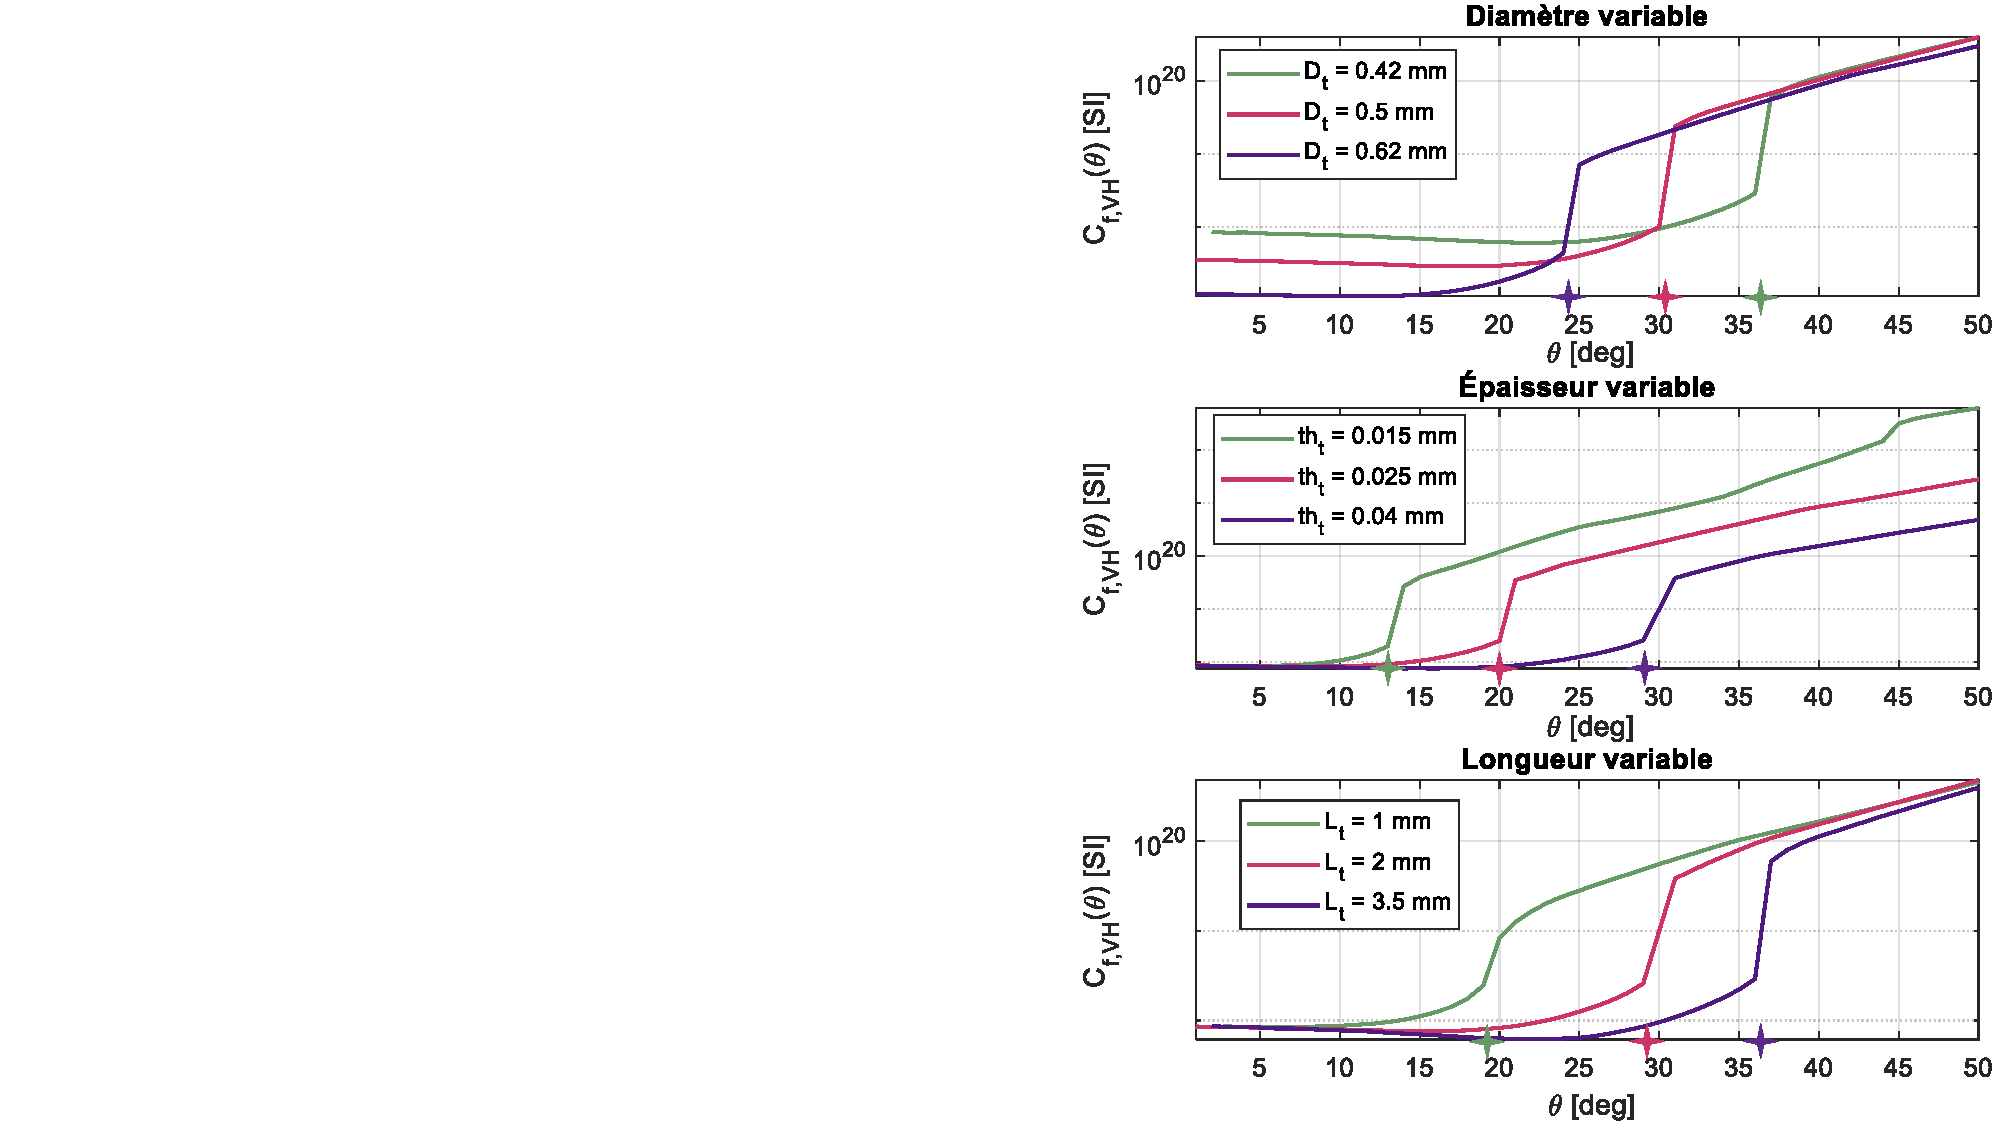
\includegraphics[trim={18cm 0cm 0cm 0cm},clip, 					                 width=0.7\textwidth]{../Chap5/Figure/prospection_Cf_L&R&thvar.pdf}
%	\caption{Impact de l'épaisseur, de la longueur et du diamètre initial du tube sur $C_{f,VH}(\theta)$}
%	\label{fig:prospection_Cf_L&R&thvar}
%\end{center}	
%\end{figure}    
%%%%%%%%%%%%%%%%%%%%%%%%%%%%%%%%%%%%% 
    		%*************	
 		\subsubsection{Aspect statique}
    		%*************
Il est important d'estimer l'évolution de $K_{VH}$ en fonction de l'angle de flexion pour prédire son influence sur le comportement de l'OB. À l'aide de l'équation \ref{eq:K_HV = 1/thetadW/dtheta} et des résultats issus des mêmes simulations par EF que nous avons traité précédemment, nous pouvons tracer l'évolution de $K_{VH}$ en fonction de $\theta$ en faisant varier les différents paramètres géométriques. Ces résultats sont présentés sur la figure \ref{fig:prospection_Khv_L_R_thvar_ZOOM}. La première ligne montre l'énergie de déformation $W_t$ accumulée dans le tube. La seconde montre la rigidité $K_{VH}$ et enfin, la troisième ligne montre une vue zoomée de $K_{VH}$ pour des angles de flexion importants.  		
%%%%%%%%%%%%%%%%%%%%%%%%%%%%
\begin{figure}[!htbp]
	\begin{center}
		\captionsetup{justification=centering}
		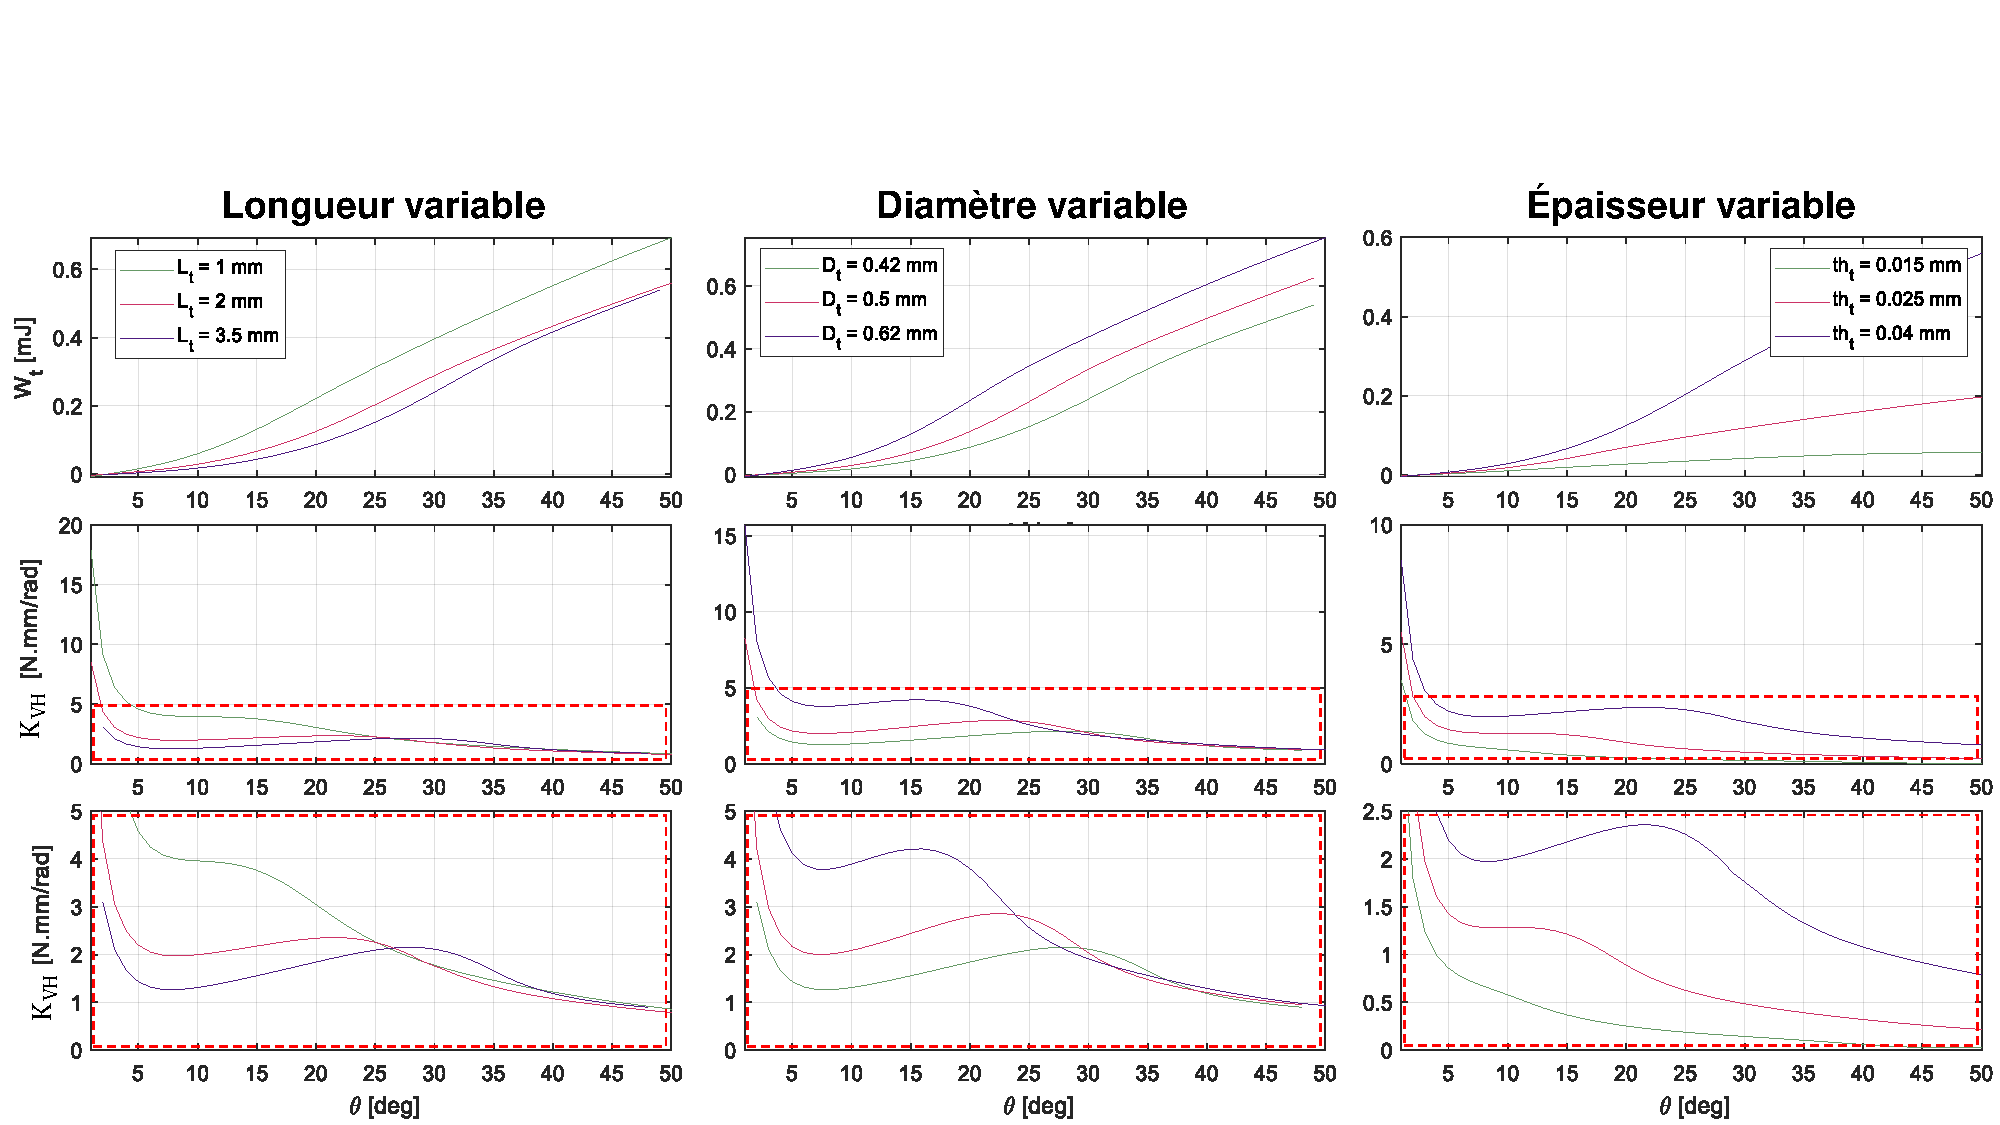
\includegraphics[trim={0cm 0cm 0cm 3cm},clip, width=\textwidth]{../Chap5/Figure/prospection_Khv_L&R&thvar_ZOOM.pdf}
		\caption{Influence de l'épaisseur, de la longueur et du diamètre initial du tube sur $K_{VH}(\theta)$}
		\label{fig:prospection_Khv_L_R_thvar_ZOOM}
	\end{center}
\end{figure} 
%%%%%%%%%%%%%%%%%%%%%%%%%%%

Les faibles épaisseurs et diamètres semblent favoriser une diminution de $K_{VH}$. De plus, le diamètre initial semble avoir un effet sur la différence de raideur pour des angles de flexion faibles. À l'inverse de l'influence sur $f_D$, il semblerait aussi que l'augmentation de $L_t$ soit favorable à la diminution de $K_{VH}$. Cela reste en accord avec le fait qu'il faut minimiser le bras de levier de pliage $a$ pour limiter l'influence de la rigidité du tube sur l'OB.

Par ailleurs, après l'apparition du flambement, $K_{VH}$ semble tendre vers une valeur unique, quel que soit le diamètre initial, ou bien la longueur du tube. Le seul paramètre, dont la faible variation influence considérablement l'évolution de $K_{VH}$ à cette échelle, reste l'épaisseur du tube. 
    %///////////////////////////////////////////// 		
	\subsection{Conclusions de l'étude EF}
    %/////////////////////////////////////////////	
L'optimisation d'une VH, de façon à ce qu'elle respecte le cahier des charges hydraulique et énergétique, impose de concevoir un tube dont :
\begin{itemize}[label=$\circ$]
	\item La réduction de $f_D$ à la section flambée se fait pour un $\Delta \theta$ le plus faible possible et permet d'atteindre le rapport de fermeture $(r_{Cf})_{min}=10$ grâce au coefficient de PdC ainsi généré.
	\item La rigidité $K_{VH}$ est la plus faible possible pour minimiser son impact sur la dynamique de l'OB.
\end{itemize}
Les observations faites en traitant les informations de l'étude EF ont été les suivantes :
\begin{itemize}[label=$\bullet$] 
	\item $(r_{Cf})_{min}$ est facilement atteignable dans chacun des triplets de paramètres considérés.
	\item $K_{VH}$ est d'autant plus grand que le diamètre $D_t$ et la longueur $L_t$ du tube augmentent, pour des angles de flexion faibles avant le flambement. Après flambement, $D_t$ et $L_t$ tendent à n'avoir que très peu d'influence sur les deux critères de conception énoncés ci-dessus.
	\item L'évolution décroissante de l'épaisseur du tube est l'évolution majeure qui tend à favoriser le respect des deux critères. 
	\item La variation de $f_D$ est très faible avant le flambement, comparée à son évolution post-flambement.
\end{itemize}
En considérant ces observations, on peut établir une méthode pour dimensionner et concevoir le tube adapté au système que nous avons pré-dimensionné avec le niveau énergétique considéré dans le chapitre \ref{ch:2_Modelisation et simulation du systeme}.
    %///////////////////////////////////////////// 		
	\subsection{Choix du tube d'après le modèle théorique}
	\label{sec:5.2.4_Choix du tube d apres le modele theorique}
    %/////////////////////////////////////////////	
L'OB a été dimensionné et conçu à partir des données des simulations préliminaires du modèle système sur Matlab-Simulink (sous-sec. \ref{subsec:2.5.3:Simulation et resultats}). Dans un premier temps, il s'agira donc de chercher un tube dont les caractéristiques mécaniques et hydrauliques peuvent être intégrées au modèle. On rappelle notamment que $x_0=0.49$mm est le niveau de flambement de l'OB sans VH.

Nous avons étudié leurs comportements mécaniques et établi un modèle analytique de pertes de charges pour vérifier si les tubes kapton existants sont adaptés à notre application. Les tubes considérés sont issus du même catalogue fournisseur que ceux testés dans l'approche expérimentale. Le \emph{''candidat''} qui remplit les critères du CdC est un tube Kapton de diamètre intérieur $D_{T40}=0.3$mm et d'épaisseur $th_{T40}=0.015$mm qu'on nomme par sa référence T40.
%%%%%%%%%%%%%%%%%%%%%%%%%
\begin{figure}[!htbp]
	\begin{center}
		\begin{subfigure}[b]{0.48\textwidth}
			\captionsetup{justification=centering}
			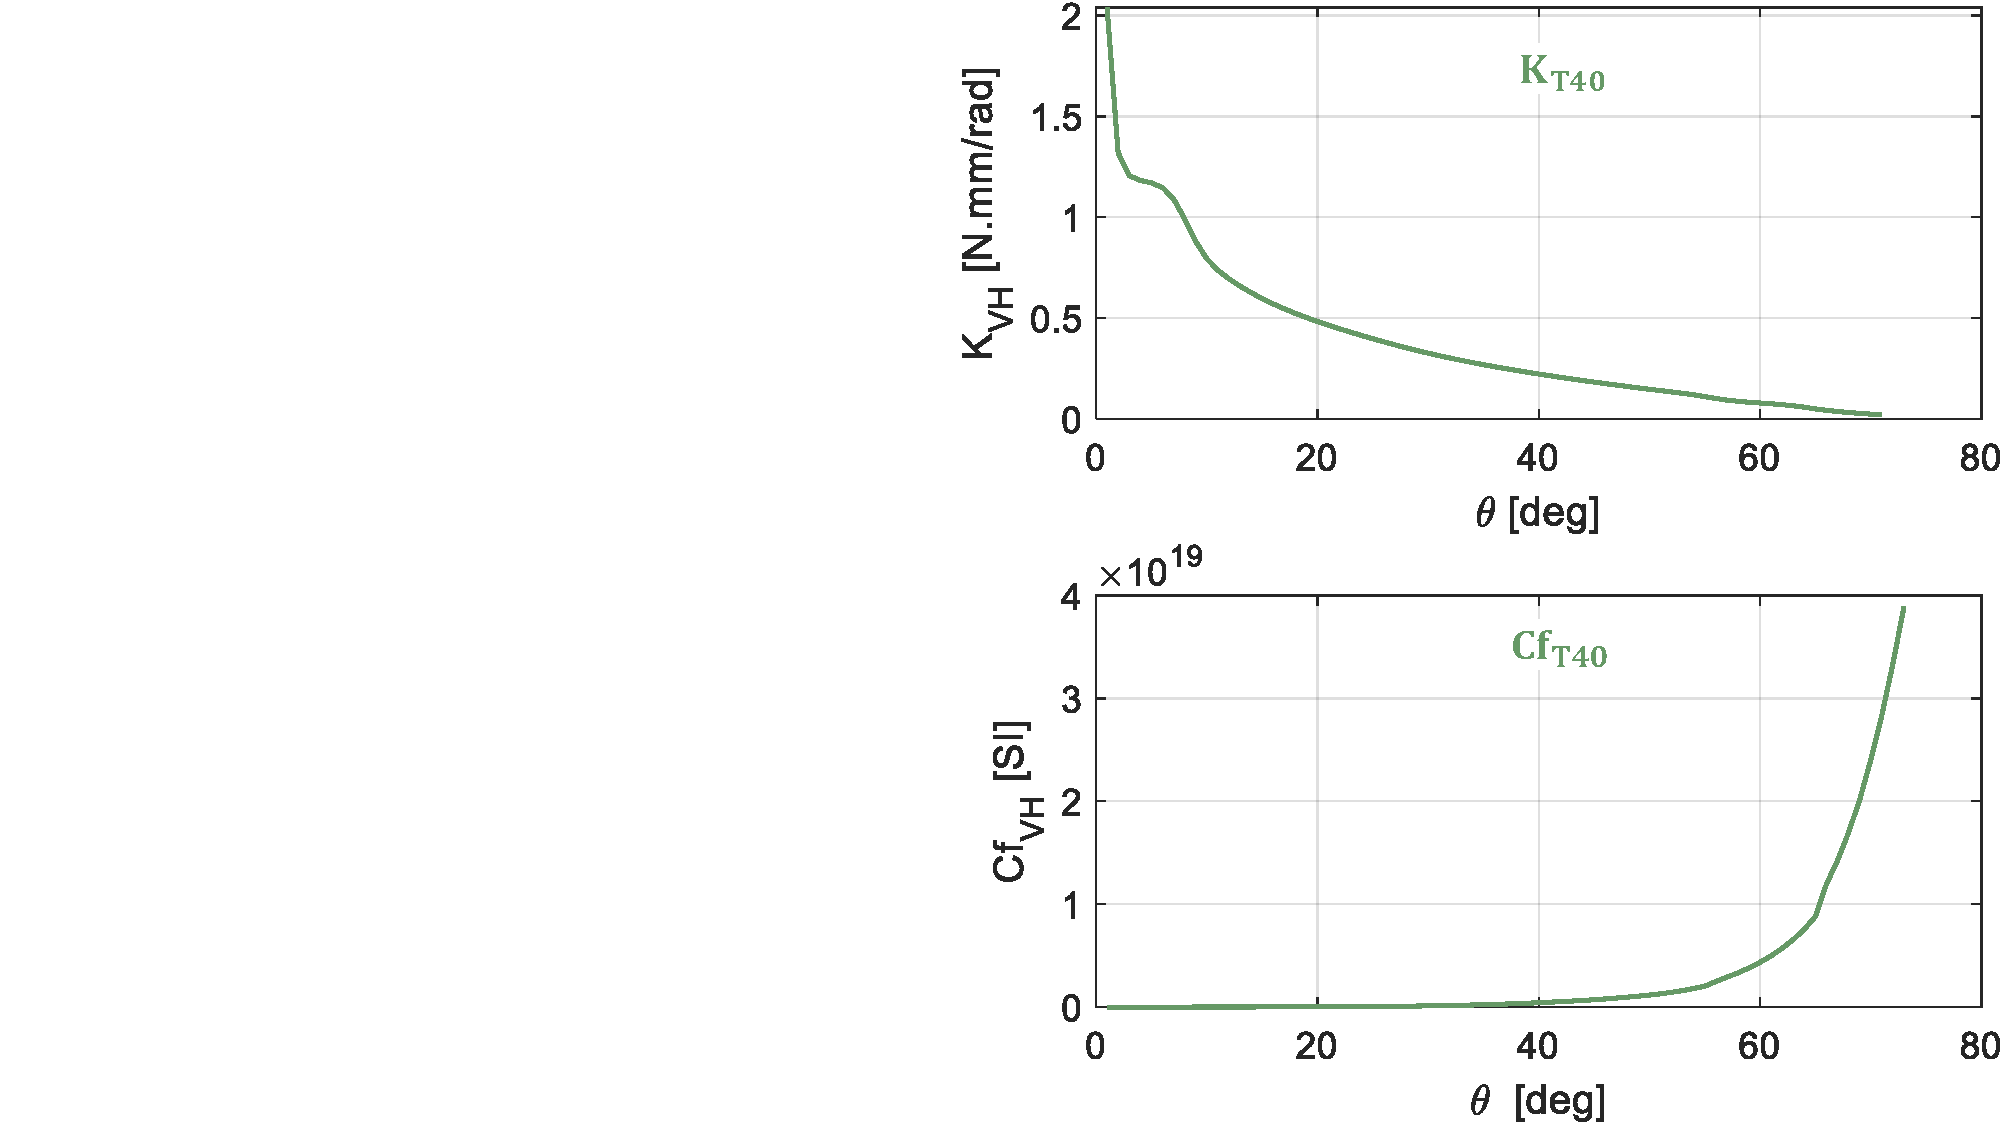
\includegraphics[trim={16cm 0cm 0cm 0cm},clip,width=\textwidth]{../Chap5/Figure/(K_VH)_(Cf_VH)_vs_theta.pdf}
			\caption{Pour tous les angles $\theta_{T40}$ simulés en EF}
			\label{fig:(K_VH)_(Cf_VH)_vs_theta}
		\end{subfigure}
		\hfillx
		\begin{subfigure}[b]{0.48\textwidth}
			\captionsetup{justification=centering}
			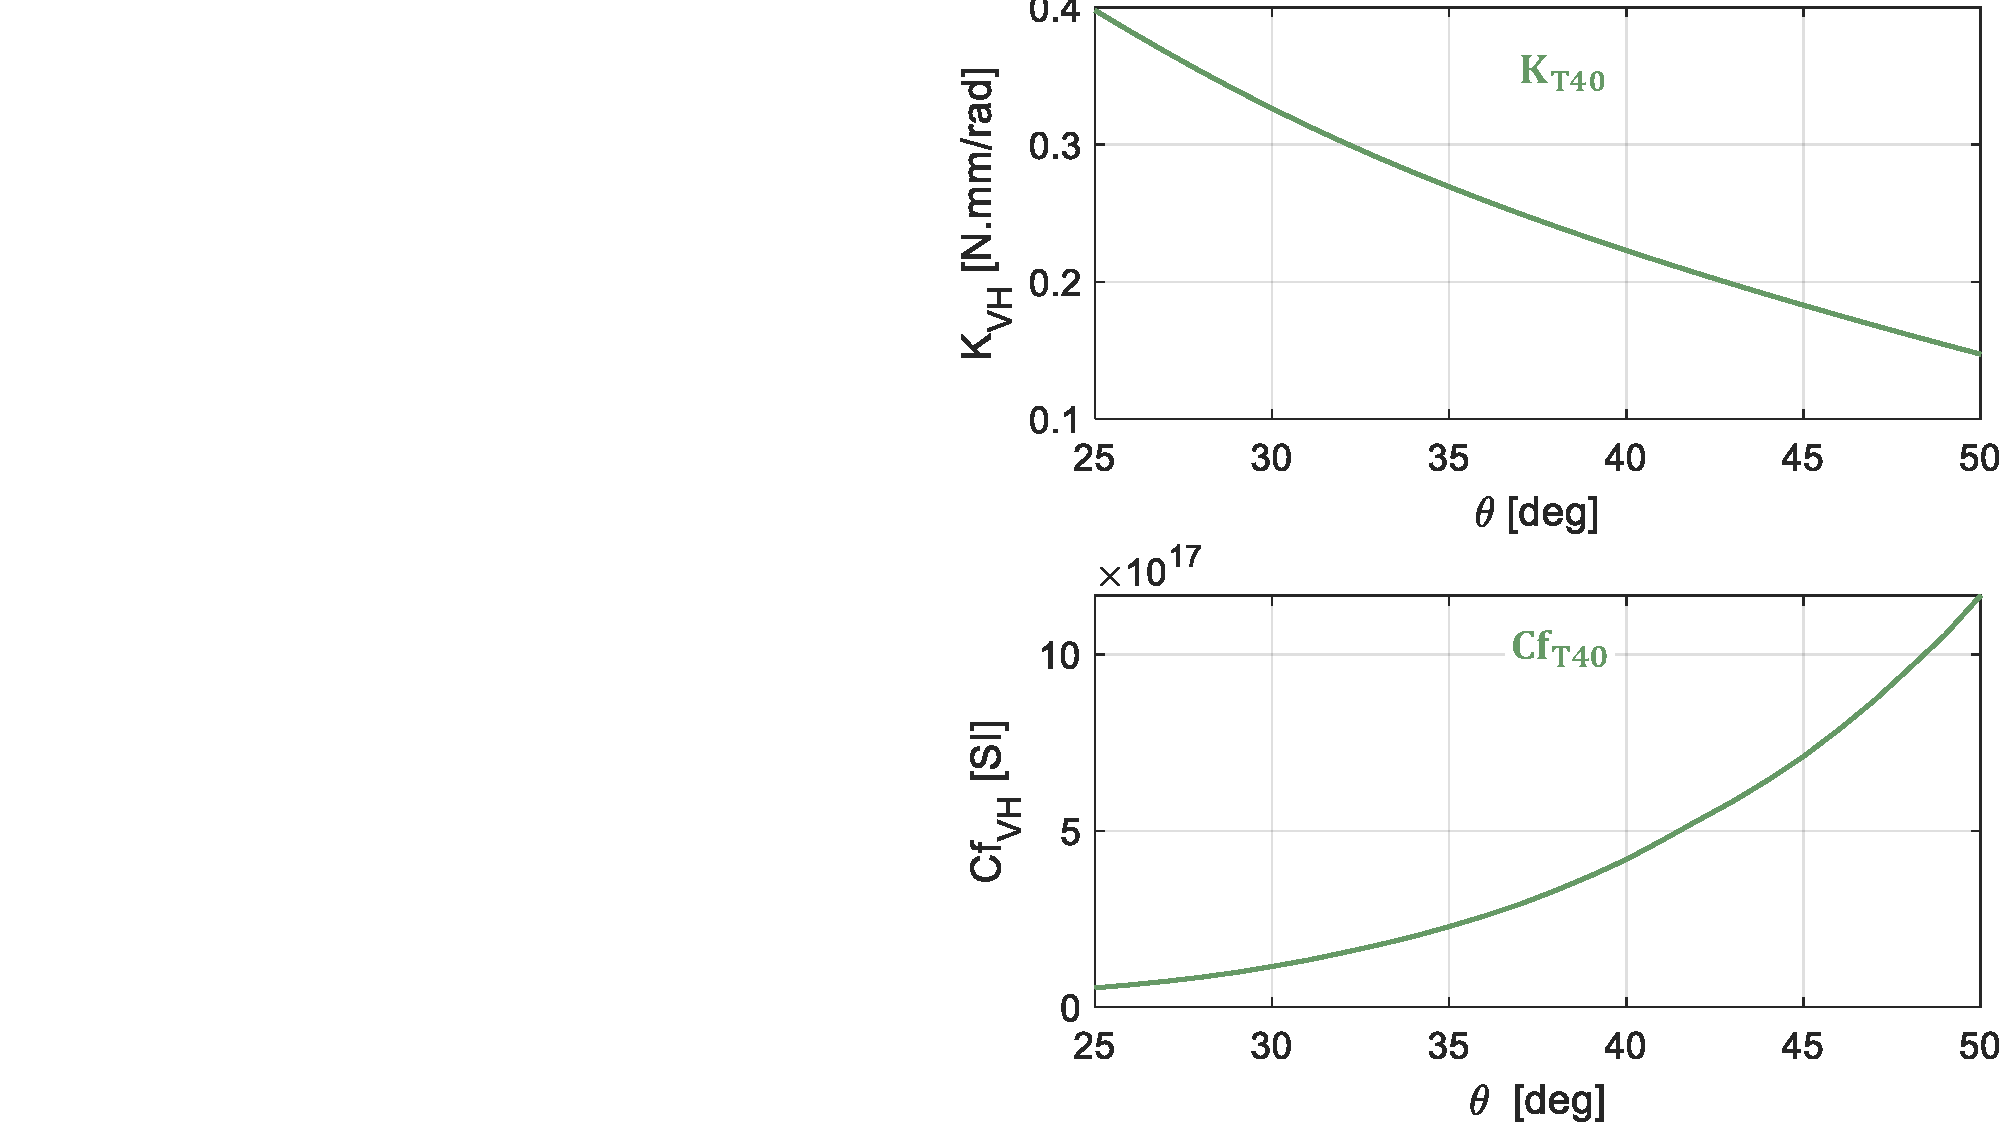
\includegraphics[trim={16cm 0cm 0cm 0cm},clip,width=\textwidth]{../Chap5/Figure/(K_VH)_(Cf_VH)_vs_theta_25-50.pdf}
			\caption{Pour $\theta \in \Delta \theta _{25,50}$}
			\label{fig:(K_VH)_(Cf_VH)_vs_theta_CdC}
		\end{subfigure}
		\caption{Évolution de $K_{T40}$ et $Cf_{T40}$ en fonction de $\theta_{T40}$}
		\label{fig:K_T40 et Cf_T40}
	\end{center}
\end{figure}
%%%%%%%%%%%%%%%%

La rigidité théorique en flexion $K_{T40}$, ainsi que le coefficient de perte de charge $Cf_{T40}$ induit dans la section flambée du tube T40, sont présentés sur la figure \ref{fig:(K_VH)_(Cf_VH)_vs_theta}. Ces résultats sont obtenus grâce au modèle de simulation par EF présenté précédemment, couplé à l'équation \ref{eq:Cf_definition}. Comme on a pu constater précédemment, la rigidité du tube baisse rapidement après le flambement, qui pour le tube T40 se produit autour de \ang{10}. Il serait donc intéressant d'utiliser le tube dans une plage d'angles post flambement afin de diminuer considérablement $K_{VH}$. Cela pourra être réalisé expérimentalement en intégrant à la VH une butée mécanique similaire à celle qu'on a présentée dans l'étude expérimentale (fig. \ref{fig:presentation_BDT_lacher_tube}).

Plusieurs choix sont possibles pour la plage de fonctionnement de la VH, dans la mesure où on s'assure que le critère de restriction hydraulique permettant d'obtenir le rapport minimal $(r_{Cf})_{min}$ est respecté. Il est à privilégier un angle d'ouverture $\theta_0$ le plus faible possible afin de limiter les PdC dans la branche qui actionne l'OB. En accord avec les CdC hydraulique, on peut utiliser le tube sur la plage d'angle $\Delta \theta _{25,50} = \theta \in [\ang{25};\ang{50}]$ comme plage de fonctionnement. L'évolution de $K_{T40}$ et $Cf_{T40}$ sur cette plage d'angle est présentée sur la figure \ref{fig:(K_VH)_(Cf_VH)_vs_theta_CdC}.  Le rapport de fermeture $r_{Cf,T40}=17$ sur $\Delta \theta_{25,50}$, et donc est supérieur à $(r_{Cf})_{min}$. Le tube T40 valide donc le critère hydraulique du fonctionnement. Aussi, la raideur du tube T40 sur $\Delta \theta _{25,50}$ est du même ordre de grandeur que celle du tube T100p (fig. \ref{fig:(K_VH)_vs_theta_D1mm_plastifie}) dont le comportement statique a été validé expérimentalement. En ce sens, il est théoriquement possible d'intégrer le tube T40 de diamètre $D_{T40}=0.3$mm et d'épaisseur $th_{T40}=0.015$mm comme VH sur l'OB fabriqué.

Nous allons regarder dans quelle mesure les outils théoriques développés dans ce chapitre sont aptes à prédire les résultats expérimentaux.
%/!\/!\/!\/!\/!\/!\/!\/!\/!\/!\/!\/!\/!\/!\/!\/!\/!\/!\/!\/!\/!\/!\/!\/!\ 
\section{Corrélations modèle - essais du comportement des VH}
\label{sec:5.3}
%/!\/!\/!\/!\/!\/!\/!\/!\/!\/!\/!\/!\/!\/!\/!\/!\/!\/!\/!\/!\/!\/!\/!\/!\
Dans cette section, les résultats expérimentaux des tubes T50,T100,T200 et T300 (tab. \ref{tab:dim_tube_statique}) seront confrontés aux modèles EFs conformes à leurs dimensions respectives. Il s'agira d'évaluer la justesse du modèle de tubes flexibles face aux données expérimentales sur les aspects statiques et hydrauliques.
    %///////////////////////////////////////////// 		
	\subsection{Comportement statique}
	\label{subsec:5.3.1_Comportement statique}
    %/////////////////////////////////////////////	
La plastification locale n'a pas été introduite dans le modèle EF. Cette action induit un changement majeur dans le comportement mécanique du matériau. La comparaison des résultats de simulation se fera donc avec les résultats expérimentaux sans plastification. Sur la figure \ref{fig:resultats_essais_statique_VH_tous_simu_vs_non_plastife}, les résultats issus des méthodes de EF et les relevés expérimentaux sont tracés en superposition, respectivement pour chacun des tubes T50, T100, T200 et T300. Le tableau \ref{tab:dim_tube_statique_simu/exp} donne les valeurs des paramètres respectifs des tubes simulés et des tubes testés expérimentalement.

Le modèle théorique prédit une rigidité d'un ordre de grandeur cohérent avec les résultats issus des essais expérimentaux. La rigidité calculée par EF est cependant bien plus importante pour les angles de départ, comparé aux essais. Ce phénomène peut être causé par les différences entre le modèle théorique et la réalité.

Expérimentalement, $L_t$ est choisie de façon à faciliter la fabrication, la caractérisation et l'intégration du tube en tant VH sur l'OB. Lorsque $D_t$ et $th_t$ sont imposés, l'angle maximal, pour lequel le modèle EF converge, dépend de $L_t$. Ce-dernier est donc choisi pour maximiser cet angle. La figure \ref{fig:prospection_Khv_L_R_thvar_ZOOM} montre alors que la rigidité théorique pour les angles faibles est d'autant plus importante que la longueur du tube simulé est faible, ce qui est le cas pour tous les tubes testés (tab. \ref{tab:dim_tube_statique_simu/exp}).

D'autre part, les conditions aux limites du modèle théorique supposent aucun contact par un objet extérieur et le centre de rotation $O$ reste fixe pour tous les angles. En condition expérimentale, lorsque le support entre en contact avec le tube, celui ci fléchit jusqu'au flambement et le centre de rotation se décale alors légèrement à chaque incrément d'angle. Ceci résulte du fait que la flexion est en partie reprise par la portion du tube kapton que nous supposons fixe. En conséquence,  expérimentalement la raideur en rotation du tube est plus faible du point de vue du support.

De plus, les données matériau présentées sur la figure \ref{fig:Dupont_kapton} nous informent sur le comportement assouplissant du Kapton dès lors qu'il est soumis à des contraintes. Les simulations prédisent un ordre de grandeur de 100MPa sur la contrainte subie à la section flambée, ce qui d'après la courbe matériau devrait baisser le module d'élasticité autour de 2GPa.

Enfin, la méthode de fabrication des tubes, par le fournisseur, consiste à enrouler une feuille de kapton sur elle-même en spirale et utiliser un adhésif pour assurer l'étanchéité. Le comportement matériau du modèle EF ne prend, lui, pas en compte les hétérogénéités ainsi créées par la méthode de fabrication initiale des tubes.

Néanmoins, compte tenu du fait que nous souhaitons utiliser les VH sur une plage d'angles de flexion se situant après l'apparition du flambement, la proximité relative des résultats du modèle, avec ceux obtenus expérimentalement, le rendent pertinent et utile pour un pré-dimensionnement.
%%%%%%%%%%%%%%%%%%%%%%%%%%%%%%%%%%%%	
\begin{figure}[!htb]
	\begin{center}
		\captionsetup{justification=centering}
		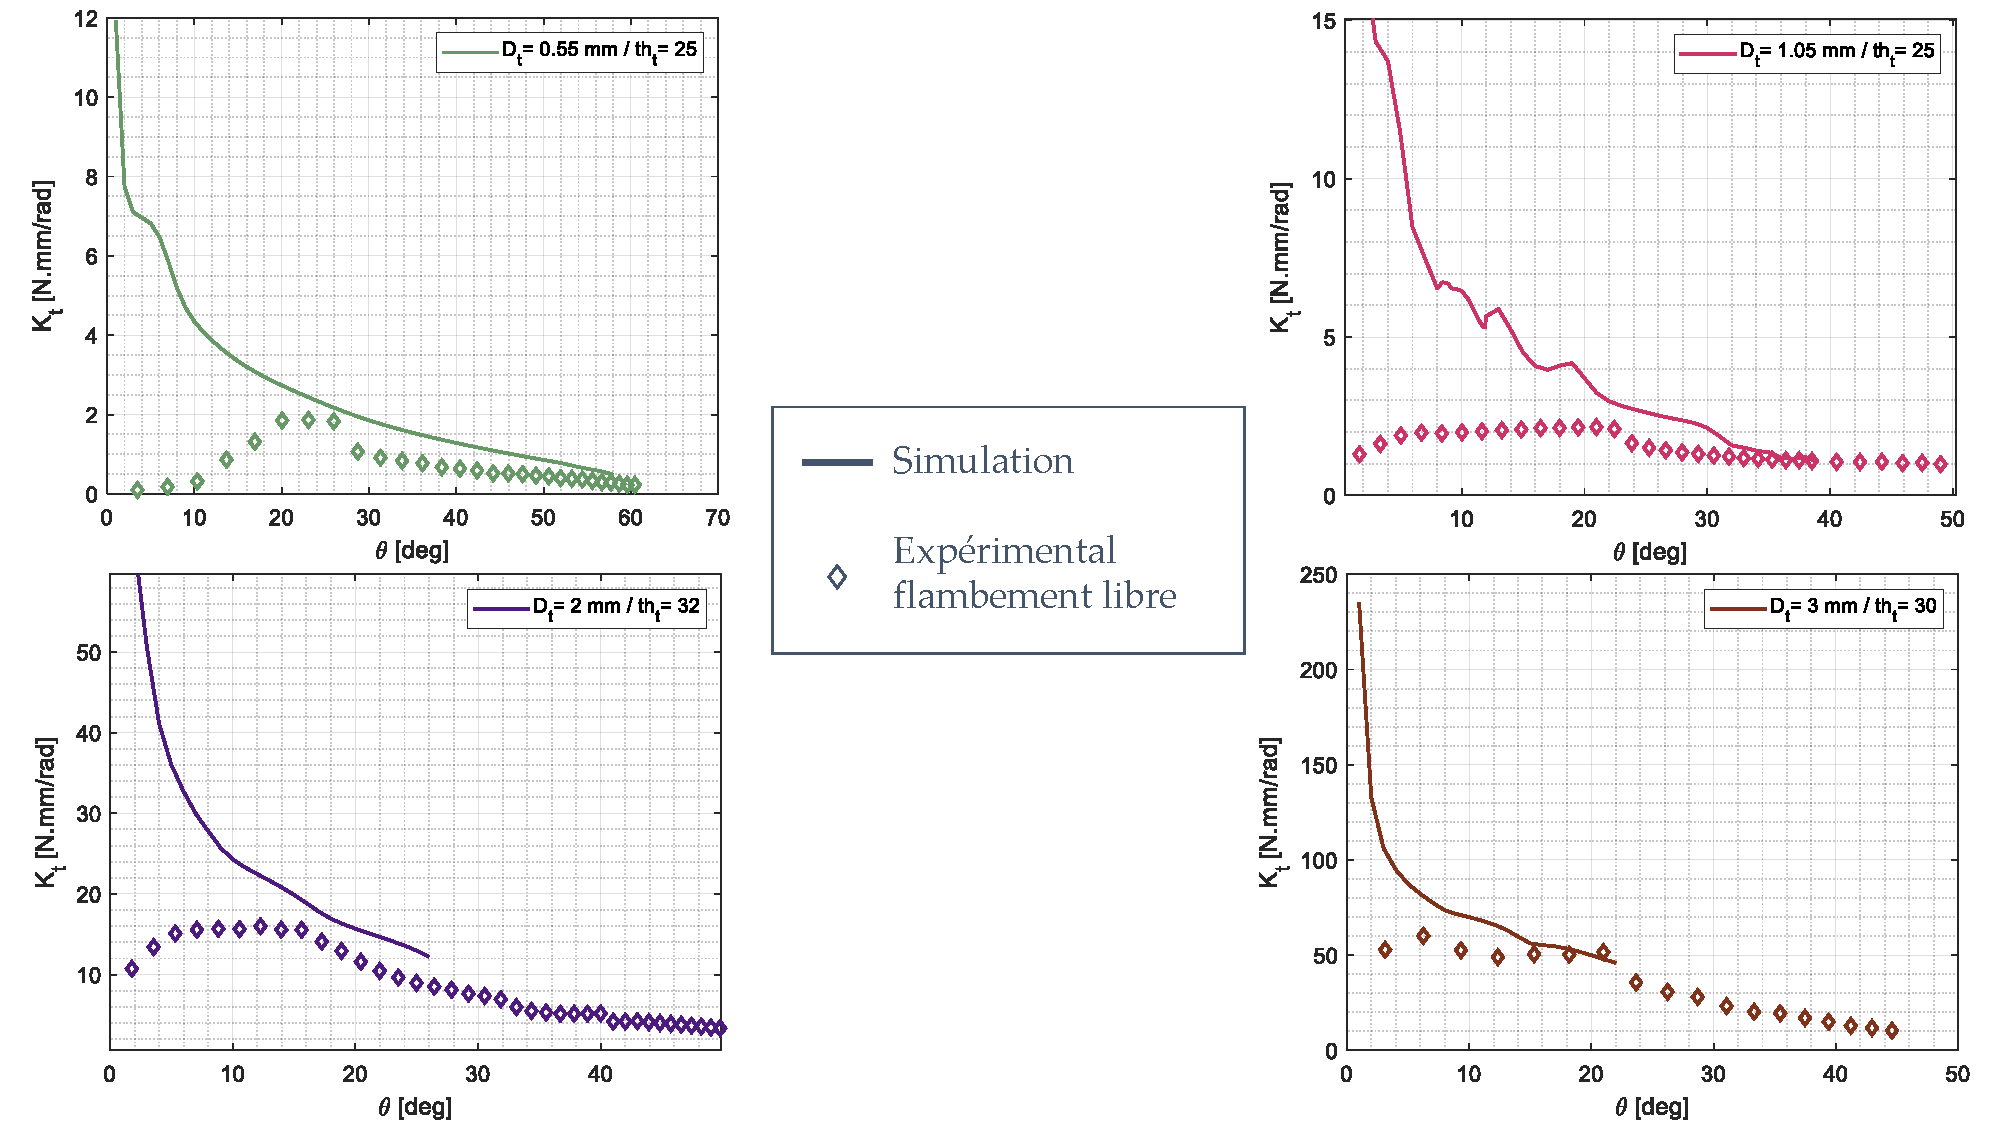
\includegraphics[trim={0cm 0cm 0cm 0cm},clip,width=\textwidth]{../Chap5/Figure/resultats_essais_statique_VH_tous_simu_vs_non_plastife.pdf}
		\caption{Évolutions théoriques et expérimentales de $K_t$ en fonction de $\theta$ }
		\label{fig:resultats_essais_statique_VH_tous_simu_vs_non_plastife}
	\end{center}
\end{figure} 
%%%%%%%%%%%%%%%%%%%%%%%%%%%%%%%%%%%% 
%%%%%%%%%%%%%%%%%%%%%%%%%%%%%%%%%%%%	
\begin{table}[!htbp]
	\centering
		\begin{tabular}[t]{|c||c|c|c|c|c|c|c|c|}
\hline
\multirow{2}{*}{\textbf{Paramètre}} &
\multicolumn{2}{|c|}{\textbf{T50}} & 
\multicolumn{2}{|c|}{\textbf{T100}} & 
\multicolumn{2}{|c|}{\textbf{T200}} & 
\multicolumn{2}{|c|}{\textbf{T300}} \\
\cline{2-9} 
& \multicolumn{1}{|c|}{Théorie} & \multicolumn{1}{|c|}{Exp.} & 
  \multicolumn{1}{|c|}{Théorie} & \multicolumn{1}{|c|}{Exp.} &
  \multicolumn{1}{|c|}{Théorie} & \multicolumn{1}{|c|}{Exp.} &
  \multicolumn{1}{|c|}{Théorie} & \multicolumn{1}{|c|}{Exp.} \\
\hline \hline
$D_t$ [mm] & \multicolumn{2}{|c|}{0.55} & \multicolumn{2}{|c|}{1.05} & \multicolumn{2}{|c|}{1.99} & \multicolumn{2}{|c|}{3} \\
\hline
$th_t$ [$\micro$m] & \multicolumn{2}{|c|}{25} & \multicolumn{2}{|c|}{25} & \multicolumn{2}{|c|}{32} & \multicolumn{2}{|c|}{30} \\
\hline
$L_t$ [mm]  &  0.8  &  1.9  &  1  &  3  & 3.9  &  5.8  &  4.4  &  11.1 \\
\hline
$D_t/th_t$ [ ] &\multicolumn{2}{|c|}{22} & \multicolumn{2}{|c|}{42} & \multicolumn{2}{|c|}{62} & \multicolumn{2}{|c|}{100} \\
\hline
$L_t/D_t$ [ ]  &  1.5  &  3.5  &  1  &  3  &  2   &  2.9  &  1.5  &  3.7 \\
\hline
$L_t/th_t$ [ ] &   32  &   76  &  40 & 120 &  122 &  181  &  147  &  370 \\
\hline
		\end{tabular}
        \caption{Dimensions des tubes testés sur le banc expérimental statique et ceux des modèle EF respectifs}
        \label{tab:dim_tube_statique_simu/exp}
\end{table}     
%%%%%%%%%%%%%%%%%%%%%%%%%%%%%%%%%%%%	
    %///////////////////////////////////////////// 		
	\subsection{Comportement hydraulique}
	\label{subsec:5.3.2_Comportement hydraulique}
    %/////////////////////////////////////////////	
On a pu voir que pour les angles faibles, notamment avant le flambement, l'évolution théorique de $C_{f,VH}$ n'est pas significative (fig. \ref{fig:prospection_Cf}). En regardant l'image rapprochée du tube T100p (fig. \ref{fig:plastification_tube}), on voit apparaître un angle initial induit par le pincement. Celui-ci est évalué à environ \ang{10} et ne semble pas induire un changement de section significatif. Par conséquent, son influence sur le comportement hydraulique du tube est considéré négligeable. Il devient alors acceptable de comparer le modèle théorique du tube T100 avec les données expérimentales du tube T100p sur leurs comportements hydrauliques respectifs.
%%%%%%%%%%%%%%%%%%%%%%%%%
\begin{figure}[!htbp]
\begin{center}
	\begin{subfigure}[h]{0.48\textwidth}
    	\captionsetup{justification=centering}
		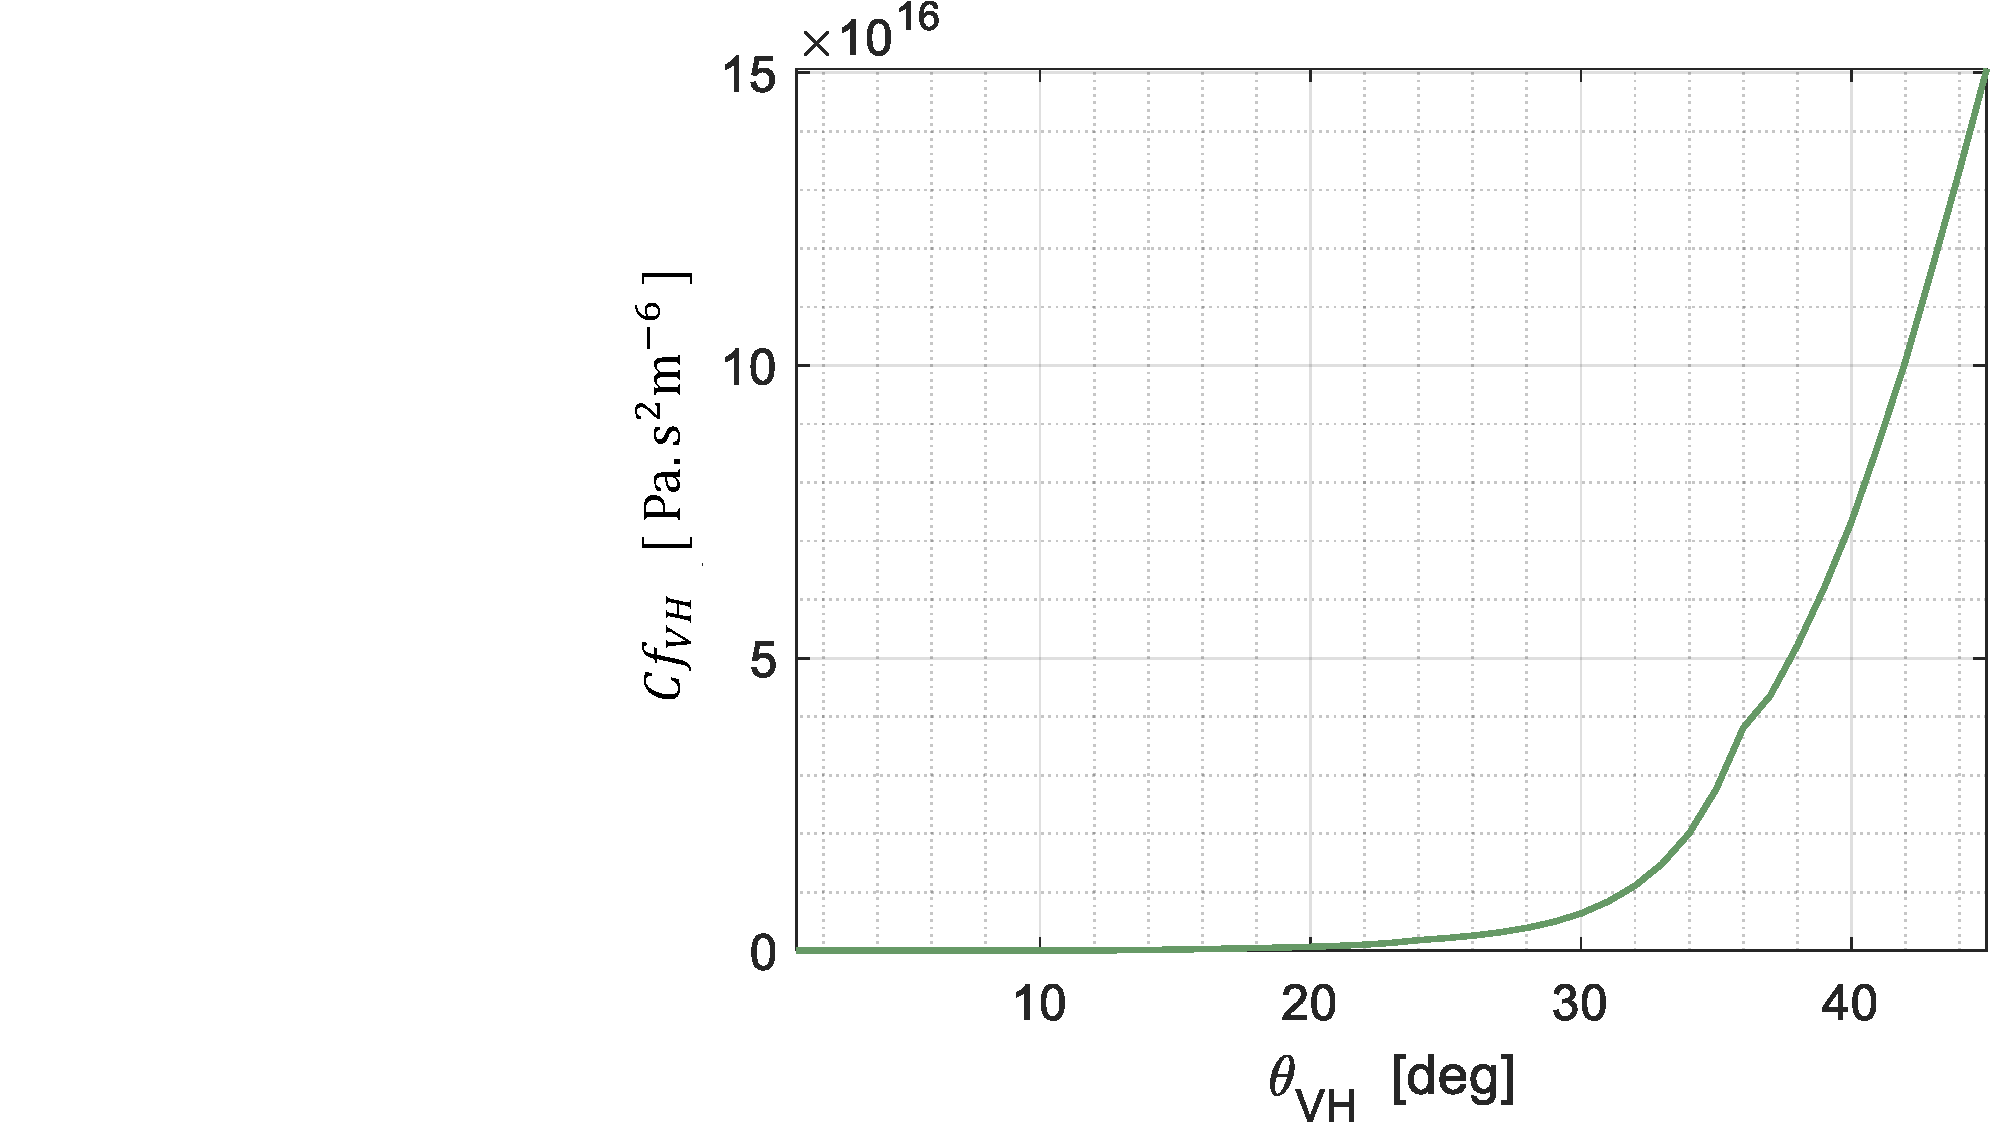
\includegraphics[trim={10cm 0cm 0cm 0cm},clip, 					                 width=\textwidth]{../Chap5/Figure/(Cf_VH)_vs_theta_D1mm.pdf}
		\caption{Simulation EF couplée au modèle analytique pour le tube T100}
		\label{fig:theorique_Cf_VH(theta)_D1mm_comparaison}  
	\end{subfigure}
\hfillx
	\begin{subfigure}[h]{0.48\textwidth}
    	\captionsetup{justification=centering}
		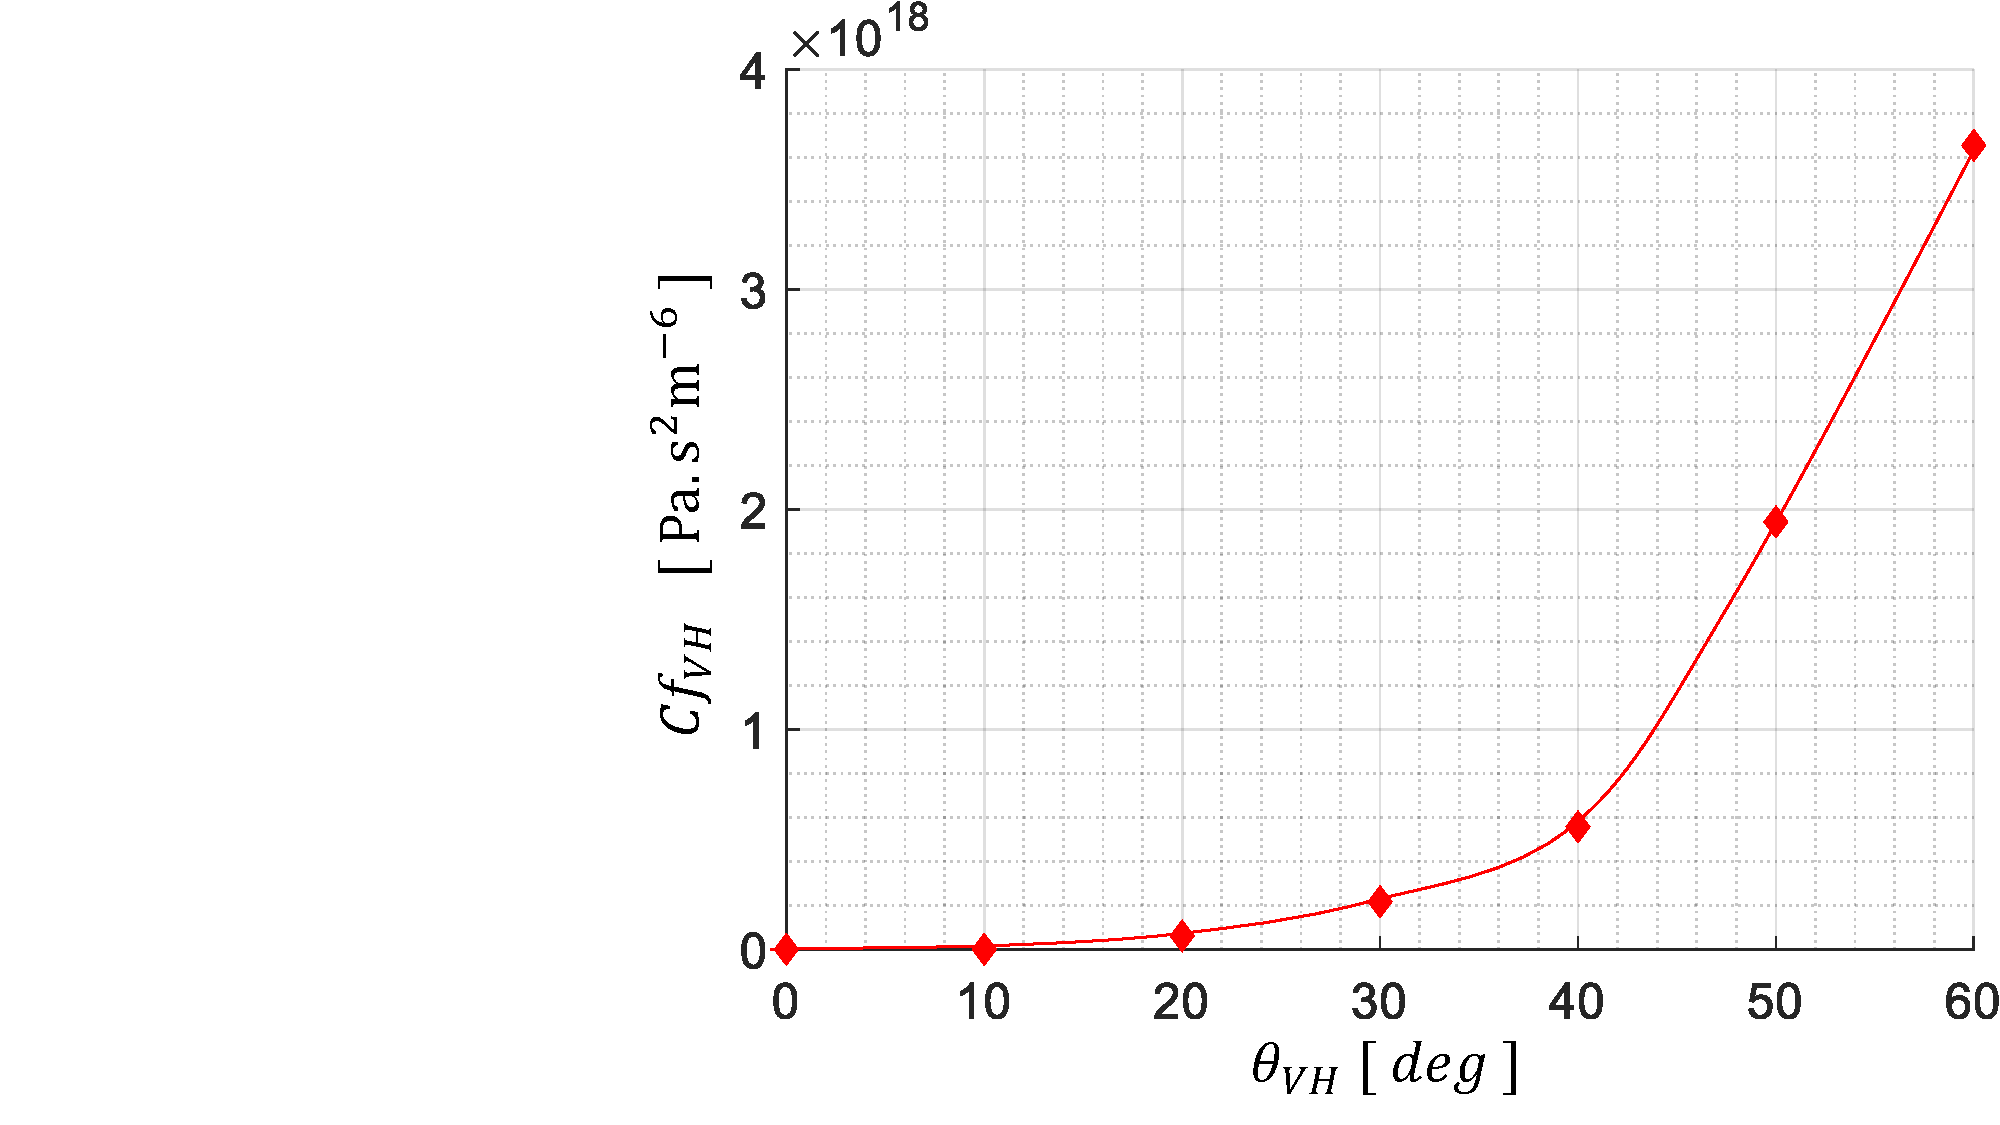
\includegraphics[trim={10cm 0cm 0cm 0cm},clip, 					                 width=\textwidth]{../Chap4/Figure/resultats_essais_hydraulique_VH_D1mm.pdf}
		\caption{Essais expérimentaux\\~~}
		\label{fig:experimental_Cf_VH(theta)_D1mm_comparaison}  
	\end{subfigure}
	\caption{Modèle théorique et expérimental de $Cf_{VH}$ pour le tube T100p}
	\label{fig:Cf_comparaison_theorie_experimental}
\end{center}	
\end{figure}
%%%%%%%%%%%%%%%%

La figure \ref{fig:theorique_Cf_VH(theta)_D1mm_comparaison} montre la courbe théorique de $Cf_{VH}$ extraite du modèle EF couplé au modèle analytique de la géométrie approximée. On trouve, en parallèle sur cette même figure, les résultats des essais expérimentaux réalisés sur le tube T100p et présentés dans le chapitre précédent. La tendance de l'évolution de $Cf_{VH}$ semble proche entre les deux jeux de données, mais la comparaison fait apparaître une différence de deux ordres de grandeur. La tendance est dictée par la fermeture de la VH et donc son effet est clairement remarquable sur les deux courbes. Les écarts peuvent cependant être causés par plusieurs facteurs.

Tout d'abord, la méthode de fabrication de la VH (fig. \ref{fig:fabrication_tube_experimental}) peut induire des singularités importantes qui ne sont pas détectables à l'\oe{}il nu et qui, au vu de l'échelle des dimensions, induisent de fortes perturbations de pression qui ne sont pas prises en compte pour l'extraction de $Cf_{VH}$. Par exemple, la jonction et l'étanchéité entre le tube et les adaptateurs(fig. \ref{fig:fabrication_tube_experimental}) est assurée par une colle peu visqueuse dont on exploite la forte capacité adhésive et les effets capillaires pour assurer le bon scellement de la valve. Un surplus d'adhésif peut former une obstruction à l'intérieur de l'échantillon de VH. De plus, la mise en place de la valve sur le plateau rotatif induit des contraintes de torsion qui sont difficiles à compenser à cause de la souplesse du kapton face à la forte rigidité du reste du circuit hydraulique. On pourra par exemple voir, sur l'image rapprochée de la VH apparaissant sur la figure \ref{fig:essais_hydraulique_VH}, la conséquence sur la géométrie qui n'est alors plus totalement cylindrique.

Par ailleurs, l'approximation géométrique pour l'établissement du modèle analytique de $C_{f,VH}$ peut être trop loin de la réalité. En effet, la géométrie réelle est différente et, de plus, elle est composée d'un étranglement et d'un coude, qui lui, n'est pas pris en compte dans le modèle analytique. Il pourrait être intéressant, de ce fait, de coupler de façon linéaire l'influence du changement de direction avec le modèle de contraction/expansion afin de les confronter aux résultats expérimentaux.

Les PdC induites par la mise en série de plusieurs singularités géométriques proches ne peuvent pas être obtenues par l'ajout (linéaire) des PdC pour chacune d'elles. Il existe en effet un couplage fluide plus complexe. Des solutions peuvent alors être appliquées pour établir un modèle de PdC robuste pour un écoulement dans une section flambée. Un premier exemple serait une étude empirique des VH. Le circuit hydraulique du banc de test devra être adaptable au diamètre de la valve afin d'induire un minimum de perturbations et de ce fait aider à isoler l'influence seule de la VH en flambement. Une seconde façon de procéder serait d'établir un modèle EF de l'écoulement au travers de la section flambée que nous obtenons suite à l'étude statique. Ce modèle devra contenir les singularités géométriques du réel pour une prédiction plus juste. Enfin, il serait intéressant de corréler ces deux méthodes afin d'évaluer leurs robustesses respectives.
%/!\/!\/!\/!\/!\/!\/!\/!\/!\/!\/!\/!\/!\/!\/!\/!\/!\/!\/!\/!\/!\/!\/!\/!\ 
\section{Conclusion de l'approche théorique}
%/!\/!\/!\/!\/!\/!\/!\/!\/!\/!\/!\/!\/!\/!\/!\/!\/!\/!\/!\/!\/!\/!\/!\/!\ 
Une approche théorique a été présentée dans ce chapitre, pour le dimensionnement des VH à base de tubes flexibles flambés. Afin d'établir un modèle de PdC approché en fonction des paramètres géométriques du tube, une approximation sur la géométrie de la section flambée a été réalisée. Un modèle EF a aussi été établi pour étudier le comportement de la section flambée pour un mouvement de flexion imposé. Le modèle théorique révèle que le tube T40 de diamètre $D_{T40}=0.3$mm et d'épaisseur $th_{T40}=0.015$mm est viable comme VH sur l'OB fabriqué d'après les CdC hydraulique et statique.

La corrélation entre le modèle théorique et les études expérimentales de la VH à base de tube T100 a été présentée. Les similarités sur le comportement statique post-flambement ont été soulignés entre les deux modèles. Les différences sur les deux aspects hydrauliques et statiques ont été relevés et des pistes de réflexion sur les causes potentielles ont été émises. Enfin, des pistes d'améliorations ont été données pour ajuster le modèle théorique afin de le rapprocher de la réalité. Des remarques ont aussi été formulées concernant l'amélioration du banc expérimental hydraulique.

À ce stade du développement du modèle, l'approche par simulations semble prometteuse, car elle donne les bonnes tendances et les bons ordres de grandeurs en ce qui concerne la raideur en rotation des tubes. En revanche, les résultats ne sont pas suffisamment proches de la réalité pour être exploitables pour un dimensionnement. En conséquence, dans le chapitre suivant, les données utilisés pour compléter le modèle système comprenant le comportement des VH, seront ceux obtenus expérimentalement avec le tube T100p.

	 
	 
%On peut alors regrouper les termes faisant intervenir $f_D$ dans l'équation \ref{eq:Cf_Gibson_fD} pour l'exprimer comme le produit d'une fonction dépendant de $\theta$ et d'une fonction dépendant de $f_D$ avec l'équation \ref{eq:Cf_Gibson_produit_fonctions_fD}. 
%\begin{equation}
%C_{f,VH}  = 
%	\frac{4\ \rho}{\pi^2\ {f_D}^4\ {D_t}^4}\
%	\Biggl[ 1.6(1-{f_D}^2)^{0.75} + 5.2(1-{f_D}^2)^2 
%	\Biggr] sin(\theta)
%\label{eq:Cf_Gibson_produit_fonctions_fD}
%\end{equation} 
%On sait que . On peut estimer son influence sur l'évolution de $C_{f,VH}(f_D)$.
%L'étranglement causé par le flambement sera d'autant plus grand que l'évolution $f_D$ en fonction de $\theta$ sera importante. On peut alors écrire :
%\begin{equation}
%\begin{split}
%\text{ODG}(C_{f,VH}) &\ =\ \text{Cst}\ \cdot \ \text{ODG}(D_h)^{-4}\ \cdot \ (10\text{ODG}(f_D)^{1.5} + 20\text{ODG}(f_D)^4)\\
%		      &\ =\ \text{Cst}\ \cdot\ \text{ODG}(D_h)^{-4}\ \cdot \ \text{ODG}(f_D)^{6.5}
%\end{split}
%\end{equation}
%Où Cst est l'ordre de grandeur des termes constants restants. On sait qu'au vu de l'application, les diamètres en jeu devraient se trouver dans l'$ODG$ du millimètre. aussi, le rapport $f_D$ se trouvant entre 0 et 1, on pourra l'estimer à $10^-1$. On peut alors comparer l'impact que ces deux termes auront sur $C_{f,VH}$ en estimant le rapport suivant:
%\begin{equation}
%	\frac{\text{ODG}(D_h)^{-4}}{\text{ODG}(f_D)^{6.5}}\ =\ \frac{(10^{-3})^{-4}}{(10^{-1}){6.5}}\ \approx\ 10^5
%\end{equation}